\documentclass[12pt]{report}
%this is for left,right,top,right margin
\usepackage{enumerate}
\usepackage{geometry}
\usepackage{mathptmx}
\usepackage{graphicx}
\usepackage{fancyhdr}
\usepackage{titlesec}
\pagestyle{myheadings} \setcounter{secnumdepth}{3} \setcounter{tocdepth}{3}
\renewcommand{\bibname}{\normalfont\fontsize{14pt}{0pt}\selectfont\bfseries REFERENCES}
\renewcommand{\listfigurename}{\fontsize{14pt}{0pt}\selectfont LIST OF FIGURES}
\renewcommand{\listtablename}{\fontsize{14pt}{0pt}\selectfont LIST OF TABLES}
\renewcommand{\thesection}{\fontsize{14pt}{0pt}\selectfont\arabic{section}}
\titleformat{\section}{\normalfont\fontsize{14pt}{0pt}\bfseries}{\thesection}{1em}{}
\titleformat{\subsection}{\normalfont\fontsize{12pt}{0pt}\bfseries}{\thesubsection}{1em}{}
\titleformat{\subsubsection}{\normalfont\fontsize{12pt}{0pt}\bfseries}{\thesubsubsection}{1em}{}



\geometry{
        a4paper,
        total={170mm,257mm},
        top=35mm,
        left=35mm, right=20mm,
        bottom=20mm
}
\renewcommand{\baselinestretch}{1.5}
\renewcommand{\contentsname}{\fontsize{14pt}{0pt}\selectfont TABLE OF CONTENTS}

\fancypagestyle{myheadings}
\fancyhf{}
\fancyhead{}
\fancyfoot{}
\fancyhead[R]{\thepage}
%\fancyhead[LE]{\thepage}
\renewcommand{\headrulewidth}{0pt}
\renewcommand{\footrulewidth}{0pt}
\rhead{\thepage}
\pagestyle{fancy}

\makeatletter
\renewcommand\tableofcontents{%
        \if@twocolumn
        \@restonecoltrue\onecolumn
        \else
        \@restonecolfalse
        \fi
        \section*{\contentsname
                \@mkboth{%
        \MakeUppercase\contentsname}{\MakeUppercase\contentsname}}%
        \@starttoc{toc}%
        \if@restonecol\twocolumn\fi
}
\renewcommand\listoffigures{%
        \if@twocolumn
        \@restonecoltrue\onecolumn
        \else
        \@restonecolfalse
        \fi
        \section*{\listfigurename
                \@mkboth{%
        \MakeUppercase\listfigurename}{\MakeUppercase\listfigurename}}%
        \@starttoc{lof}%
        \if@restonecol\twocolumn\fi
}

\renewcommand\listoftables{%
        \if@twocolumn
        \@restonecoltrue\onecolumn
        \else
        \@restonecolfalse
        \fi
        \section*{\listtablename
                \@mkboth{%
        \MakeUppercase\listtablename}{\MakeUppercase\listtablename}}%
        \@starttoc{lot}%
        \if@restonecol\twocolumn\fi
}


\renewenvironment{thebibliography}[1]
{\section*{\bibname}% <-- this line was changed from \chapter* to \section*
        \@mkboth{\MakeUppercase\bibname}{\MakeUppercase\bibname}%
        \list{\@biblabel{\@arabic\c@enumiv}}%
        {\settowidth\labelwidth{\@biblabel{#1}}%
                \leftmargin\labelwidth
                \advance\leftmargin\labelsep
                \@openbib@code
                \usecounter{enumiv}%
                \let\p@enumiv\@empty
        \renewcommand\theenumiv{\@arabic\c@enumiv}}%
        \sloppy
        \clubpenalty4000
        \@clubpenalty \clubpenalty
        \widowpenalty4000%
\sfcode`\.\@m}
{\def\@noitemerr
        {\@latex@warning{Empty `thebibliography' environment}}%
\endlist}


\makeatother

\newenvironment{nscenter}
{\parskip=0pt\par\nopagebreak\centering}
{\par\noindent\ignorespacesafterend}
\begin{document}
\pagenumbering{roman}
\newpage
\pagenumbering{gobble}
\begin{figure}[t]
        \centering
        
\includegraphics[width=50mm]{resources/tu-logo.jpg}
\end{figure}
\begin{nscenter}
        TRIBHUVAN UNIVERSITY\\ 
        INSTITUE OF ENGINEERING\\
        CENTRAL CAMPUS, PULCHOWK\\
        \vspace{21mm}
        \bfseries{
                MUSIC CLASSIFICATION BASED ON GENRE AND MOOD\\
        }
        \vspace{14mm}
        \textbf {Submitted By:}\\
        \textnormal{
                Ayush Shakya\hspace{25mm}[069/BCT/505]\\
                Bijay Gurung\hspace{25mm}[069/BCT/512]\\
                Mahendra Singh Thapa\hspace{9mm}[069/BCT/519]\\
                Mehang Rai\hspace{28mm}[069/BCT/524]\\
        } 
        \vspace{18mm}
        \textnormal{
                A PROJECT WAS SUBMITTED TO THE DEPARTMENT OF ELECTRONICS
                AND COMPUTER ENGINEERING IN PARTIAL FULLFILLMENT OF THE REQUIREMENT
                FOR THE BACHELOR’S DEGREE IN COMPUTER ENGINEERING\\
                \vspace{17mm}
                (August, 2016)
        }
\end{nscenter}

\newpage
\pagenumbering{Roman}
\setcounter{page}{2}

\newpage
\section*{COPYRIGHTS}
\addcontentsline{toc}{section}{\numberline{} COPYRIGHT}

The author has agreed that the Library, Department of Electronics and Computer Engineering, Pulchowk Campus, Institute of Engineering
may make this report freely available for inspection. Moreover, the author has agreed that permission for extensive copying of this project
report for scholarly purpose may be granted by the supervisors who supervised the project work recorded herein or, in their absence, by the
Head of the Department wherein the project report was done. It is understood that the recognition will be given to the author of this report
and to the Department of Electronics and Computer Engineering, Pulchowk Campus, Institute of Engineering in any use of the material of this
project report. Copying or publication or the other use of this report for financial gain without approval of to the Department of Electronics
and Computer Engineering, Pulchowk Campus, Institute of Engineering and author’s written permission is prohibited.\\
Request for permission to copy or to make any other use of the material in this report in whole or in part should be addressed to:\\
Head\\
Department of Electronics and Computer Engineering\\
Pulchowk Campus, Institute of Engineering\\
Lalitpur, Kathmandu\\
Nepal\\



\newpage
\section*{ACKNOWLEDGMENT}
\addcontentsline{toc}{section}{\numberline{} ACKNOWLEDGMENT}

It has been a great pleasure to work with different individuals whose perpective and ideas has directly or indirectly assisted or motivated us. 
We would like to gratitude to everyone whose ideas lead to this completion of the project. It is a matter of fact a great privilege for us to 
acknowledge their assistance and contributions to our project.\\
\\
First and foremost, we would like to express our sincere gratitude towards Dr. Basanta Joshi, our supervisor under whose supervision there was successful completion of our project. Without his
invaluable guidance and suggestions, it would have been a difficult journey for us. His useful suggestions for this whole work and cooperative
behavior are sincerely acknowledged.\\
\\
We would like to thank the Department of Electronics and Computer Engineering for adding this major project as part of final year curriculum
and hence giving us this opportunity to undertake the project. The great need of research, time and sheer coding has allowed us to harness our
skills, experience and knowledge.\\ 
\\
We are also grateful to Dr. Nanda Bikram Adhikari for letting us carry out this project and co-operating with us to carry out the project smoothly. We would like to thank and express our gratitude  to all out
respective subject teachers for sharing their precious knowledge, constant support and guidance.\\
\\
Last but not the least, we would like to thank our friends for motivating us and providing numerous assistance throughout the project development duration.\\




\newpage
\section*{ABSTRACT}
\addcontentsline{toc}{section}{\numberline{} ABSTRACT}

This report describes and documents all the aspects and working functionality of our final year project titled “Music Classification System
Based on Genre and Mood”. The project is part for the curriculum for the subject Major Project under the course of final year of B.E. in Computer Engineering.
As the title itself describes the overall aim of the project is to develop a system capable of classifying music based on Genre and mood, with the availability of large
number of digital media and the disorder introduced being the primary motivation.\\  
\\
The methodology used is that of a modular system consisting of two main stages. The first stage involves the preprocessing of the raw audio
data resulting in the extraction of a number of features pertaining to music signal: Intensity, MFCC, rhythm, pitch. Each feature extractor
reduces the information content in the raw data to a vector in a small number of dimensions. Or in other words we can say that feature extractor 
analyses the music signal and extracts its respective features compatible for further processing. It requires intensive knowledge of digital signal
analysis and processing, signal sampling,etc. The second stage comprises of all the machine learning portion. In it, the set of feature vectors are classified(indexed) into certain clusters
by the use of certain algorithms: K-means, Support Vector Machines and  Artificial Neural Networks. This technically requires knowledge of all those respective algorithms.\\ 
\\
This report also documents our approach towards the system development following the various aspects of Software Engineering. UML diagrams have been
used to model the entire system and ERD diagrams have been used to show the relationship between the various entities in our system and iterative 
development method was chosen for the development of our system. Java language along with spring framework was used to build our whole system along
with the GUI.\\




\clearpage
\thispagestyle{fancy}
\addcontentsline{toc}{section}{\numberline{} TABLE OF CONTENTS}
\tableofcontents
\thispagestyle{fancy}
%\newgeometry{left=3.5cm,top=3.5cm,right=2cm,bottom=2cm}

\newpage
\addcontentsline{toc}{section}{\numberline{} \listfigurename}
\listoffigures{\thispagestyle{fancy}}

\newpage
\addcontentsline{toc}{section}{\numberline{} \listtablename}
\listoftables{\thispagestyle{fancy}}
%\restoregeometry

\newpage
\section{INTRODUCTION}
\pagenumbering{arabic}

\subsection{Background}

Music can be literally defined as the combination of soothing sounds. A more complex definition of music can be: an amalgam of 
melody, harmony, rhythm, timbre and silence in a particular structure. Music is an art form and cultural activity whose medium is sound and silence. It's a 
form of entertainment that puts sounds together in a way that people like or find interesting. To form music, musical instruments are not necessary,
for example: a cappella, barbershop, choral, scat, plainsong, isicathamiya, etc don't use instruments at all.
A group or a person can simply sing in rhythm and form music. Sometimes musician may use their voice to make noises similar to a musical intrument.
Music is deeply related to human emotions \cite{Juslin2001} and psyche too. It can be relaxing, invigorating or even saddening. \\
\\
The common elements of music are pitch (which governs melody and harmony), rhythm (and its associated concepts tempo, meter, and articulation),
dynamics (loudness and softness), and the sonic qualities of timbre and texture (which are sometimes termed the "color" of a musical sound). Different styles
or types of music may emphasize, de-emphasize or omit some of these elements. Music is performed with a vast range of instruments and with 
vocal techniques ranging from singing to rapping, and there are solely intrumental pieces, solely vocal pieces. The creation, performance, significance,
and even the definition of music vary according to culture and social context.\\
\\
The advent of music dates back to the primal years of human history. We can point it out due to the fact of presence of tribal music--like the ancient African bushman tribal song--which has been passed on
from generation to generation, Nepalese traditional/cultural song from each race,etc. 
But music can be complex not only due to its origins but also due to the evolution of music in different technological era. 
We have seen the evolution of music from legendary classical Beethoven symphonies to modern day hiphop which is widely popular among the youths nowadays. We have seen the rise of different genres like classical, rock,
pop, metal,etc. and there are countless others too and many more are sure to be born. For example, The advent of the Techno Genre is pretty recent.\\
\\
It is unlikely for a single person to listen to each and every genre present out there let alone all those songs. Every person may acquire a different taste 
in music. Some may like clasical music while come may like rock music, it's based on their choice. So a person may probably only distinguish a particular unknown song 
if those song were to belong to his/her genre of choice and the same goes for the mood. So realising this problem, there has been a increasing amount of research
and work done in the music sector for the automatic classification of song based on genre. Though classification based on genre has been a popular one,
classification based on mood catching the sight of many people lately.\\
\\
With the advent of networks and internet, the number of songs are increasing exponentially throughout the internet. Website like soundcloud, youtube, facebook,etc. 
has given a platform for people to pursue their interest in music by forming like groups, composing and releasing songs, sharing songs,etc.
Internet has made it possible for worldwide connection of whole world and it has harnessed the music industry. Because of internet only the
popularity of music artists has been increasing all around the world. Their music have now been able to reach each and every corner of the world.
This freedom of music throughout the internet has lead to increasing amount of songs and their databases.
Due to these rapid development in the music industry, there has been an increasing amount of work in the area of automatic genre classification
of music in audio format. A serious factor behind this automation can be considered as the increasing number of millions of records by different 
artist every year. A simple automation in classification would be much suited than a hand-to-hand task by human and its applicability can be huge.
Moreover, there might be conflict regarding genre and mood issue based on the perception of a human being. So regarding these
issues MIR(Music Information Retrieval) has primarily focused on automation of classification of such music based on signal analysis. Such systems
can be used as a way to evaluate features describing music content as well as a way to structure large collections of music.\\


\subsection{Overview}
Throughout the evolution of music, the music industry took a different path and the difference in nature, flow of music, it's tempo, etc. is 
huge and quite complicated. It lead to the evolution of different numerous genre. The presence of numerous genre is a source of confusion and more often
than not people are overwhelmed with the sheer vastness of music available. We humans can most of the times easily categorize simple song based on genre
or mood by simply listening and analysing few sample of similar song based on similarity but we are never truly able to understand its nature or
features distinction. So we can sometimes never able to recognize them correctly in case of genre and mood. There are songs out there for
example Bohemian Rhapsody, which we can never really point it out to a distinct genre and mood.\\
\\
Moreover the advent of internet has escalated the popularity of music and various artists. Nowadays everyone wants to be a singer. They want to become famous.
So, various sites like soundcloud, youtube, facebook,etc. has provided them the perfect platform for sharing their songs. Not only for some novice
singers but also for whole popular artist and whole music industry it has provided the perfect platform for sharing the music and growing itself.
This has lead to release of millions of songs and increase in database of the system. So given the today world in computerized technological era,
automation is nowadays seen as a popular subject in every field. There is being development of automation in every field like riding cars, manufacturing factories,
etc. This popularity has affected the music industry too. Realising the potential of its applicability, there has been number of research in this sector/field.
Numbers of research paper are being published regarding the automation of classification of music with research paper \cite{Tzanetakis1992} published by George Tzanetakis and Perry Cook
being one of the first in this field with the primary motivation to make it easier for people to classify music (based on genre and/or mood)
so that they can find songs suited to their own tastes. It can also lay the foundation for figuring out ways to represent similarity
between two musical pieces and in the making of a good recommendation system.\\
\\
Given the perplexing nature of music, music classification requires specialized representations, abstraction and processing techniques for effective
analysis, evaluation and classification that are fundamentally different form those used for other mediums and tasks. So focusing on these issues
we created a music classification system which is web based application used for classifying music. We did not limit ourselves only to genre which is
the burning issue in the music industry but we made our effort for the music classification based on mood too. In music industry there is a vast
number of different genre. Most of the previous work were limited to four different genres. So, to challenge ourselves we took five different genres
for our classification system, namely:-
\begin{itemize}
        \item Classical
        \item Jazz
        \item Rock
        \item Pop
        \item Hiphop
\end{itemize}
Our application took a song as an input from the user computer and classified to its genre based on feature extracted and learning of the system.\\ \\ Similar procedure was taken for classification of song based on mood. Until now not much research were done on music classification based on mood.
So we made our classification system to classify that same song based on mood which was truly based on signal analysis and not lyrical features.
For classification based on mood, we mapped the song among two dimensions: 
\begin{itemize}
        \item Arousal 
        \item Valence
\end{itemize}
So, the Arousal and Valence level can give an overview of a song:
\begin{itemize}
        \item High Arousal, High Valence = Joyful
        \item High Arousal, Low Valence  = Angry
        \item Low Arousal, High Valence  = Content
        \item Low Arousal, Low Valence   = Depressing
\end{itemize}
So, we can say that our system first extracted the required features based on the signal analysis and it's manipulation, and then used 
those features to classify it among one of the combination of five different genres and 4  different mood using the machine learning algorithm
which is already trained on dataset.\\


\subsection{Problem Statement}
The evolution of music and its origination has presented us with many different genres. The advent and popularity of internet and networking
has escalated the market and rise of music industry. Given the popularity of music industry, thousands of new artist are emerging every year. 
People are releasing song everytime as their hooby or part-time career. So we can see there are millions of songs out there world wide and is
continuously increasing every year. Internet has huge contribution for it's rise. With that much of released songs, the size of database is also 
increasing every year. Since the subject of genre and mood depends on people's perception, it has really been a tedious job to create a quite standard 
one.\\ 
\\
So we built a music classification system based on genre and mood. The choice of these genres is based on their being sufficiently distinguishable from each other.
Choosing some genre that’s very unique and abnormal might have made them more distinguishable and easier to classify but it would have been harder
to find quality data/works for those genre. So, we chose these genre with availability of musical pieces in mind too. We chose to work on 
classification based on mood too because not many work had been done in the past regarding this field. But we can see this field has a wide 
scope of applicability. It can be used as a song recommendation system based on genre and that typical mood which the user is listening
too as it is certain that the user will possibly like similar song with the similar melody. For now we are currently trying to tackle the issue of
music classification based on genre and mood and not abiding to its applications. 


\subsection{Motivation}
The presence of numerous number of different genres has presented tedious job for music industry. It has become
a source of confusion and more often than not people are overwhelmed with the sheer vastness of music available.
So, the primary motivation is to make it easier for people to classify music based on genre. Not only
genre but classification based on mood has also now intrigued many people. Combined these two will provide 
or make a solid foundation for figuring out ways to represent similarity between two musical pieces and build a good recommendation
system for music lovers who are passionate about their music and also their choices.\\
\\
It can futher tackle the issue of automated music database management with large number.  It can especially be useful 
in those cases with unknown label-genre and mood. Music player developers can then be able to make a smart playlist based on the genre 
and mood of some samples of song the user was currently or recently listening to. This would save a lot of time of user who had to
otherwise manually maintain his/her playlist everytime based on his current mood and genre of choice.

\subsection{Aims and Objectives}
\begin{itemize}
        \item To classify a music according to genre and mood.
        \item To create a web based application for music classification based on genre and mood.
        \item To extend the compatibility of the system with different types of music formats like wav,au,etc. along with mp3 format.
\end{itemize}

\subsection{Scope of Project}

This was the scope of the project as defined at the commencement.
\begin{enumerate}[(i)]
        \item The project will work on classifying music based on genre and mood. More specifcally, the classifcation will be done on western music only as the data
                is more easily available and lots of works have been done in the past for it. Also, only five genres will be used for genre classifcation:
                \begin{itemize}
                        \item Rock
                        \item Pop
                        \item Classical
                        \item Jazz
                        \item Hiphop
                \end{itemize}

            \item The mood based classification will use the two dimensional mood model based on \textit{arousal} and \textit{valence}.

            \begin{itemize}
                \item High Arousal, High Valence = Joyful
                \item High Arousal, Low Valence  = Angry
                \item Low Arousal, High Valence  = Content
                \item Low Arousal, Low Valence   = Depressing
            \end{itemize}

        \item Also, it is entirely possible for a song or a piece of music to fall into multiple genre or moods. The characteristics that defne the genre
                and the mood may change within the song itself with one part showing seeming to belong to one class while other parts may seem to belong to
                an entirely diferent class. The project will not cover such issues. In other words, multiple-tagging will not be done.

        \item The classification will work on various music file formats like mp3, au, wav,etc.

\end{enumerate}

\subsection{Organization of Report}
This report describes and details the design and methodology of building a music classification system based on genre and method. As this report consists
documentations relating to different field during development of a standard software product, hence the whole report is effectiely broke down to seven chapters.\\
\\
Chapter one is intended to introduce the project by simply presenting a brief background of the project field which is music and music industry, the motivation which drove 
us to pursue the field, the overview of the problem statement and objective of the project and at last the scope of our project.\\
\\
Chapter two presents the literature review. It provides us the collective effort that has been done in the past in our project field. Since our
project is music classification based on genre and mood, so at first we start by brief history of human audio perception, Music Information Retrieval(MIR) and music classification.
We give a general review of past activities and research on music classification based on both genre and mood. We describe the features and procedures have been involved in such system.\\
\\
Chapter three is all about the system analysis done at perspective of software engineering. It describe about the requirement specification which is
high level requirement, functional requirement and non functional requirement. It also involves feasibility assessment which contains operational feasibility, 
technical feasibility, economic feasibility, legal feasibility and scheduling feasibility.\\
\\
Chapter four involves the methodology explaining the basic system block diagram and steps that are carried in the system like audio preprocessing, feature extraction and integration,etc.\\
\\
Chapter five describes about the system development which all the use case diagram, data flow diagram and sequence diagram. It also explains about the tools and environment used for system development.\\
\\
Chapter six involves the result and analysis process. Since our music classification is based on genre and mood, so we analyze the accuracy involved in each with each feature involved and also with 
different classifiers involved. We provide the details the all the testing and validation in it. 
\\
Finally, in chapter seven we present our conclusion. We present deduce a conclusion based on the result and analysis and give our insights on future enhancement of the system.\\
\\
Along with all these there are list of references and bibliography relating to project which is included at last. There is also appendix provided which gives all the analysis
and design diagrams which have been developed during the project.\\



\newpage
\section{LITERATURE REVIEW}

\subsection{Human Audio Perception}

The human ear is an exceedingly complex organ.  To make matters even more difficult, the information from two ears is combined in a perplexing neural network,
the human brain. \cite{smith2013}

\textit{Figure 1} illustrates the major structures and processes that comprise the human ear. The outer ear is composed of two parts, the visible flap of skin and
cartilage attached to the side of the head, and the ear canal, a tubeabout 0.5 cm in diameter extending about three cm into the head. These structures direct environmental
sounds to the sensitive middle and inner ear organs located safely inside of the skull bones. Stretched across the end of the ear canal is a thin sheet of tissue called the
tympanic membrane or eardrum. Sound waves striking the tympanic membrane cause it to vibrate. The middle ear is a set of small bones that transfer this vibration to the cochlea
(inner ear) where it is converted to neural impulses. The cochlea is a liquid filled tube roughly two mm in diameter and three cm in length.
\begin{figure}[h]
        \centering
        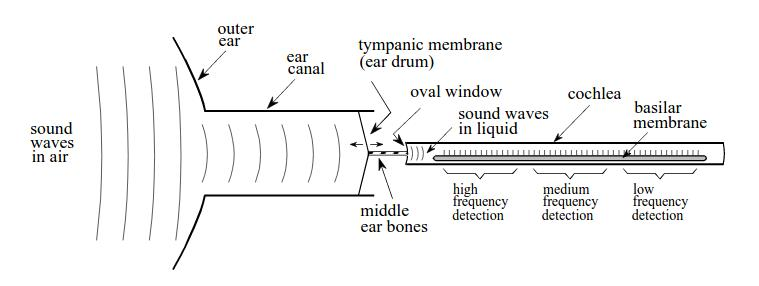
\includegraphics[width=150mm]{resources/humanear.jpg}
        \caption{Functional Diagram of Human Ear}
        \label{fig:figure1}
\end{figure}

Music can be defined as organised sound comprising the following structural elements: pitch, timbre, key, harmony, loudness (or amplitude), rhythm, meter, and tempo. Processing
these elements involves almost every region of the brain and nearly every neural subsystem.

Sound does not exist outside of the brain; it is simply air molecules moving. Sound is produced by vibrating air molecules connecting with the
eardrum at varying frequencies (pitch) and velocities (amplitude). The process starts with the brain’s primary auditory cortex receiving a signal from the eardrum/inner ear
which immediately activates our ‘primitive’ brain, the cerebellum. The cerebellum is the oldest part of the brain in evolutionarily terms and plays an important part in motor control.
It contributes to coordination, precision, and accurate timing of movements. The ear and the primitive brain are known collectively as the low-level processing units. They perform the
main feature extraction which allows the brain to start analysing the sounds, breaking down the sensory stimulus into pitch, timbre, spatial location, amplitude, reverberant environment,
tone durations, and onset times of different notes. 

This data is conducted through neurons in the brain; cells specialized in transmitting information, and the basic building blocks of the nervous system.
The output of these neurons connects to the high-level processing units located in the frontal lobe of the brain. It is important to note that this process
is not linear. The different regions of the brain constantly update each other with new information. 

\subsection{History of MIR and Music Classification}

The field of Music Information Retrieval (MIR) can be traced back to the 60s with reference to the works done by Kassler in \cite{kassler1966}.
Even Automatic Transcription of Music was attempted as early as the 70s \cite{andel1975}. However, there were two limiting factors that prevented progress in the field at the time.
Firstly, the high computational requirements of the problem domain was simply not available. 
And secondly, other related fields of study such as Digital Signal Processing, Speech Processing, and Machine Learning were also not advanced enough.  
So, the field stalled for the next few decades.

In the 1990s, the field regained prominence as computational resources improved greatly and the rise of the internet resulted in massive online music collection. So, there was both an opportunity and demand for MIR systems.
The organization of the first International Symposium on Music Information Retrieval (ISMIR 1) in 2000 highlights this resurgence of interest in the field. 
280 people from 25 different countries participated in ISMIR Conference Malaga 2015.

As for the methodologies used, MIR in the 90s was influenced by the field of Text Information Retrieval (IR), techniques for searching and retrieving text documents based on user queries.
So, most of the algorithms were developed based on symbolic representations such as MIDI files \cite{Tzanetakis2002a}. One such method is described in \cite{alghoniemy1999}.

However, as mentioned in \cite{byrd2002}, identifying approximate units of meaning in MIR, as done by the majority of text-IR methods (words serve as such units) was not easy.

Instead, statistical non-transcriptive approaches for non-speech audio signals started being adopted in the second half on the 90s \cite{Tzanetakis2002a}.
This was probably influenced by progress of such methods in other fields of speech processing. 
For example, in \cite{saunders1996}, the authors reported 98\% accuracy in distinguishing music from speech in commercial radio broadcasts.
This was based on the statistics of the energy contour and the zero-crossing rate.

In \cite{wold1996}, the authors introduced similar statistical methods for retrieval and classification of isolated sounds.
Similarly, in \cite{scheirer1997}, an algorithm for music-speech classification based on spectral feature was introduced. 
It was trained using supervised learning. 

And so, starting in the 2000s, instead of methods attempting note-level transcriptions, researchers focused on direct extraction of information of audio signals using Signal Processing and Machine Learning techniques.

Currently, three basic strategies are being applied in MIR: \cite{Casey2008}

\begin{itemize}
        \item \textbf{Based on Conceptual Metadata} - Suited for low-specificity queries.

        \item \textbf{Using High-level Descriptions} - Suited for mid-specificity queries.

        \item \textbf{Using Low-level Signal-based Properties} - Used for all specificities.

\end{itemize}

But still most of the MIR techniques being employed at present use low-level signal features instead of high-level descriptors \cite{Kaminskas2012}.
Thus, there exists a semantic gap between human perception of music and how MIR systems work.

\subsection{Audio Processing}

General Audio signal processing is an engineering field that focuses on the computational methods for intentionally altering sounds, methods that
are used in many musical applications.

\par Particularly speaking, music signal processing may appear to be the junior relation of the large and mature field of speech signal processing,
not least because many techniques and representations originally developed for speech have been applied to music, often with good results. However,
music signals possess specific acoustic and structural characteristics that distinguish them from spoken language or other nonmusical signals. \cite{muller2011}

In music the most important qualities of sound are: pitch, duration, loudness, and timbre. Duration and loudness are unidimensional, while pitch and timbre are complex and multidimensional. \cite{dooling2014}

\begin{itemize}
        \item \textbf{Loudness} - Intensity of a tone is the physical correlate that underlies the perception of loudness. Loudness variations play an important role in music, but are less important than pitch variations.

        \item \textbf{Duration} - A composer or performer can alter the pace of a piece so that its apparent (virtual) time is slower or faster than clock time. 

        \item \textbf{Timbre} - Timbre is the subjective code of the sound source or of its meaning. According to the American Standards Association, "Timbre
                is that attribute of auditory senstation of which a listener can judge that two steady-state tones having the same pitch and loudness are dissimilar."

        \item \textbf{Pitch} - Pitch is related to the frequency of a pure tone and to the fundamental frequency of a complex tone. In its musical sense, pitch
                has a range of about 20 to 5000 Hz. Some five to Zseven harmonics of a complex tone can be heard out individually by paying close attention. There
                is a dominance region for pitch perception, roughly from 500 to 2000 or 3000 Hz. Harmonics falling in the dominance region are most influential 
                with regard to pitch.

\end{itemize}

Again, these types of low dimensional features extracted from the acoustical signals are more popular than higher dimensional representations such as
Spectrograms for Classification purposes. \cite{prasad2007}

\subsection{Genre Based Classification}

\subsubsection{Overview}
Automatic Music Genre Classification (AMGC) is one of the tasks focused by MIR. However, it is not a straightforward one.

In \cite{Scaringella2006}, Scaringella et al. discuss how and why musical genres are a poorly defined concept making the task of automatic classification non-trivial.
Still, although the boundaries between genres are fuzzy and there are no well-defined definitions, it is still one of the widely used method of classification of music. 
If we look at human capability in genre classification, Perrot et al \cite{Perrot1999} found that people classified songs--in a ten-way classification setup--with an accuracy of 70\% after listening to 3s excerpts.

\subsubsection{Features}
The features used for genre based classification have been heavily influenced by the related field of speech recognition. 
For instance, Mel-frequency Cepstral Coefficients (MFCC), a set of perceptually motivated features that is widely used in music classification, was first used in speech recognition.

The seminal paper on musical genre classification by Tzanetakis et al. \cite{Tzanetakis2002} presented three feature sets for representing timbral texture, rhythmic content and pitch content. 
With the proposed feature set, they achieved a classification accuracy of 61\% for ten musical genre.

Timbral features are usually calculated for every short-time frame of sound based on the Short Time Fourier Transform (STFT). 
So, these are low-level features. 
Typical examples are Spectral Centroid, Spectral Rolloff, Spectral Flux, Energy, Zero Crossings, and the afore-mentioned Mel-Frequency Cepstral Coefficients (MFCCs).
Among these, MFCC is the most widely preferred feature \cite{Lippens2004}\cite{Kour2015}. Logan \cite{Logan2000} investigated the applicability of MFCCs to music modeling and found it to be "at least not harmful".

Rhythmic features capture the recurring pattern of tension and release in music while pitch is the perceived fundamental frequency of the sound. 
These are usually termed as mid-level features.

Apart from these, many non-standard features have been proposed in the literature. 

Li et al.\cite{Li2003} proposed a new set of features based on Daubechies Wavelet Coefficient Histograms (DWCH), and also presented a comparative study with the features included in the MARSYAS framework.
They showed that it significantly increased the accuracy of the classifier.

Anglade, Amélie, et al.\cite{Anglade2010} propose the use of Harmony as a high-level descriptor of music, focusing on the structure, progression, and relation of chords.

\subsubsection{Classification}

A variety of methods have been used for music classification. Some of the popular ones are SVM, K Nearest Neighbours and variants of Neural Networks.

The results are also widely different. In \cite{Neumayer2004}, 61 per cent accuracy has been achieved using a Multilayer Perceptron based approach. 

While in \cite{Koerich2013}, the authors have achieved 71 per cent accuracy through the use of an additional rejection and verification stage.

Haggblade et al. \cite{Haggblade2011}, compared simpler and more naive approaches (k-NN and k-Means) with more sophisticated neural networks and SVMs. 
They found that the latter gave better results.

Standard statistical pattern recognition classifiers are also used for AMGC.
They may be simple Gaussian Classifiers or Gaussian mixture model (GMM) classifier, where each class pdf is assumed to consist of a mixture of a specific number of multidimensional Gaussian distributions.
In such an approach, the parameters of each Gaussian component and the mixture weights are estimated using the iterative EM algorithm.

However, lots of unique methods -- either completely novel or a variation of a standard method -- have been put into use too. In \cite{Nasridinov2014}, the authors
propose a method that uses Chord labeling (ones and zeros) in conjunction with a k-windowSubsequenceMatching algorithm used to find subsequence in music sequence
and a Decision tree for the actual genre classification.

It is also noted that high-level and contextual concepts can be as important as low-level content descriptors. \cite{Anglade2010} 

\subsubsection{Dataset}

In \cite{Downie2003}, Downie presents the problem of a lack of a proper baseline dataset for the AMGC problem, which meant research teams couldn't scientifically compare and contrast their different approaches.

However, the publicly available GTZAN dataset introduced in \cite{Tzanetakis2002}, solved most parts of the issue by soon becoming the standard dataset used by researchers across the world.
We too used this dataset for this project.
The dataset contains 100 representative excerpts from ten different genre.
They were taken from radio, compact disks, and MP3 compressed audio files. All the files are stored as 22 050 Hz, 16-bit, mono audio files. 
The Genres dataset has the following classes: classical, country, disco, hiphop, jazz, rock, blues, reggae, pop, metal.
Among them we were only concerned with five genre as mentioned in Chapter 1: classical, hiphop, jazz, rock, and pop, So, we had a total of 500 songs in our dataset. 

\subsection{Mood Based Classification}

\subsubsection{Overview}

As mood is a very human thing, Mood Based Classification, also known as Mood Emotion Recognition (MER), requires knowledge of both technical aspects as well as the human emotional system.
So, the conceptualization of emotion and understanding of the associated emotion taxonomy is vital. However, it is a difficult thing to do, because 

a) It is subjective and 

b) We cannot agree on a model to depict emotional states.

Usually, two approaces to emotion conceptualization are taken: 

\begin{itemize}
    \item \textbf{Categorical Conceptualization} - This approach to MER categorizes emotions into a number of distinct classes. 
        It requires the belief of base emotions (happiness, anger, sadness, etc) from which all other secondary emotion classes can be derived.\cite{Ekman1992}

        However, the major drawback of the categorical approach is that the number of primary emotion classes is too small in comparison with the richness of music emotion perceived by humans.

    \item \textbf{Dimensional Conceptualization} - It defines Musical Values as numerical values over a number of emotion dimensions. 
        So, the focus is on distinguishing emotions based on their position on a predefined space.
        Most of these conceptualizations map to three axes of emotions: valence (pleasantness), arousal (activation) and potency (dominance).
        By placing emotions on a continuum instead of trying to label them as discrete, this approach can encompass a wide variety of general emotions.

\end{itemize}

\subsubsection{Circumplex and Thayer Mood Model}

One of the Dimensional conceptualization was proposed by Russell (1980) \cite{Russell1980}.
As shown in \textit{Figure 2}, the model consists of a two-dimensional structure involving the dimensions of valence and arousal. 
General emotions are placed within thic circular framework.

\begin{figure}[hlvt!]
        \centering
        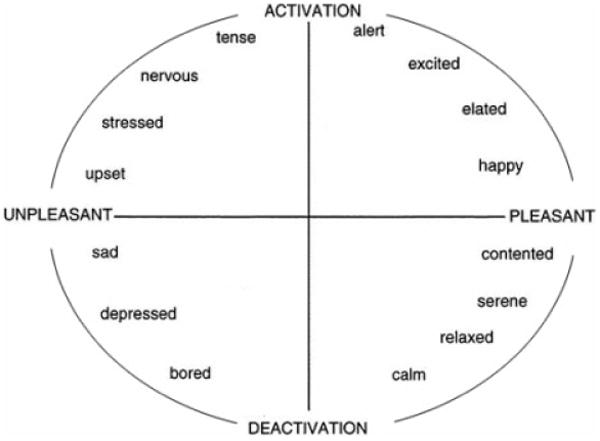
\includegraphics[width=120mm]{resources/circumplex.jpg}
        \caption{A graphical representation of the circumplex model of affect with the horizontal axis representing the valence dimension and the vertical axis representing the arousal or activation dimension.}
        \label{fig:figure2}
\end{figure}

As shown in \textit{Figure 3}, Thayer \cite{Thayer1990} proposed a similar two-dimensional approach that adopts the theory that mood is entailed from two factors: -Stress (happy/anxious) -Energy (calm/ energetic). 
This divides music mood into four clusters: Contentment, Depression, Exuberance and Anxious/Frantic.

Although, the two-dimensional approach has been criticized as deficient (leading to a proposal of the third dimension of potency), it seems to offer the right balance between sufficient "verbosity" and low complexity \cite{Juslin2001}.

\begin{figure}[hlvt!]
        \centering
        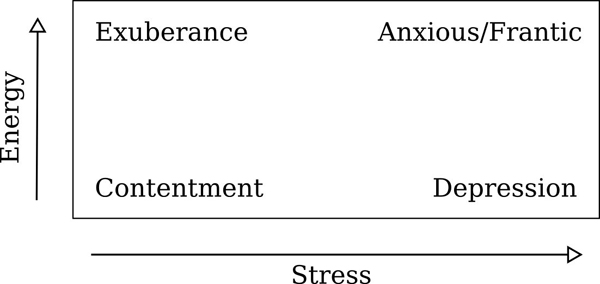
\includegraphics[width=120mm]{resources/thayerModel.jpg}
        \caption{Thayer's two-dimensional model of mood}
        \label{fig:figure3}
\end{figure}

\subsubsection{Features}

Some of the commonly used features in MER are:

\begin{itemize}
    \item \textbf{Energy}: Energy related features such as audio power, loudness, specific loudness sensation coefficients (SONE), are correlated to the perception of arousal. 
        Lu et al. \cite{Lu2006} used it to classify arousal.

    \item \textbf{Rhythm}: Flowing/fluent rhythm is associated with positive valence while firm rhythms with negative valence.

    \item \textbf{Melody}: These include features such as Pitch (perceived fundamental frequency), chromogram centroid, etc.

    \item \textbf{Timbre}: As with the AMGC problem, MFCC is widely used in MER too. Apart from MFCC, octave-based spectral contrast as well as DWCH (Daubechies wavelets coefficient histogram) are also proposed in literature.
        
\end{itemize}

So, we see that the features used in MER are almost the same as those in AMGC. However, Fu et al. note in their extensive survey on Audio-based Music Classification \cite{Fu2011} that although their effectiveness is debatable, mid-level features such as Rhythm seem to be more popular in MER.


\subsubsection{Classifiers}

The algorithms used in AMGC are also popular in MER. So, support vector machines, Gaussian mixture models, neural networks, and k-nearest neighbor are the ones regularly used.

\subsubsection{Dataset}

Due to the high variability in the emotional models adopted (whether categorical or dimensional), there have been no popular baseline dataset for MER task.

So, to tackle the issue, in 2013, Soleymani et al. \cite{Soleymani2013} created a 1000 songs dataset for emotional analysis of music which uses the Valence-Arousal axes for representing emotional values for songs.
We have used a filtered version (with some redundancies removed) of that dataset resulting in a final set of 744 songs.

The songs, in the dataset, each 45 seconds long, were collected from FMA. They used Amazon Mechanical Turk as a crowdsourcing platform for collecting more than 20,000 annotations on the 1,000 songs. 
Furthermore, their analysis on the annotations revealed a higher agreement in arousal ratings compared to the valence ratings.

\subsection{Factors affecting accuracy}
Some of the factors that affect the accuracy are: 
\begin{enumerate}[(i)] 
        \item \textbf{Multi-tagging:} A song can belong to multiple genre. So it is sure to consist of features characterizing multiple genre. This might creating a
                problem for any classification technique applied as it is sure to create ambiguity. 
        \item \textbf{Noise:} Many of the songs may not be recorded in the studio. Some may be recorded during live music while some in concert. We are sure to find
                noise in the latter cases which may tamper the original signal of music hence giving a deviated feature vector. This is sure to affect the accuracy of classification system.
        \item \textbf{Similar feature in different genre:} Some of the feature of different genres may somehow be similar in some aspects. For example: intensity of metal
                and rock are high, beat is also high in both, and so on. 
\end{enumerate}


\newpage
\section{THEORETICAL BACKGROUND}

\subsection{Features}

\subsubsection{Compactness}
It is the measure of the noisiness of a signal. It is found by comparing the 
components of a window’s magnitude spectrum with the magnitude spectrum of its  
neighbouring windows.\\ 
\\
If M[n], M[n-1] and M[n+1] $>$ 0, then
\begin{equation}
        compactness = \sum_{n=2}^{N-1}{((|20*log(M[n]))-20*(log(M[n-1])+log(M[n])+log(M[]n+1))/3|)}
\end{equation}
otherwise,
\begin{equation}
        compactness = 0
\end{equation}
where M[n] is the Magnitude Spectrum at internal n.

\subsubsection{Mel-Frequency Cepstral Coefficients}
It is a representation of the short-term power spectrum of a sound, based on a linear cosine 
transform of a log power spectrum on a nonlinear mel scale of frequency.\\
\\
\textbf{Algorithm}
\begin{enumerate}[(i)]
        \item \textbf{Framing:}
                The process of segmenting the speech samples obtained from analog to digital conversion(ADC) into a small frame with the length within
                the range of 20 to 40 msec. The voice signal is divided into frames of Nsamples. Adjacent frames are being separated by M(M $<$ N).
        \item \textbf{Hamming Window:}
                Hamming window is used as window shape by considering the next block in feature extraction processing chain and integrates all the 
                closest frequency lines. The Hamming window equation is given as:\\
                \\
                If the window is defines as W(n), 0 $\le$ n $\le$ N-1 where\\
                N = number of samples in each frame\\
                Y[n] = Output signal
                X(n) = Input signal
                W(n) = Hamming window,\\
                then the result of windowing signal is shown below:
                \begin{equation}
                        Y(n) = X(n) \times W(n)
                \end{equation}
                \begin{equation}
                        W(n) = 0.54 - 0.46cos\Big(\frac{2 \pi n}{N-1}\Big), \hspace{10mm}0 \le n \le N-1
                \end{equation}
        \item \textbf{Fast Fourier Transform:}
                To convert each frame of N samples from time domain into frequency domain. The Fourier Transform is to convert the
                convolution of the glottal pulse U[n] and the vocal tract impulse response H[n] in the time domain. This statement supports the equation below:
                \begin{equation}
                        Y(w) = FFT[h(t)*X(t)] = H(w) * X(w)
                \end{equation}
                If X(w), H(w) and Y(w) are the Fourier Transform of X(t), H(t) and Y(t) respectively.
        \item \textbf{Mel Filter Bank Processing:}
                The frequencies range in FFT spectrum is very wide and voice signal does not follow the linear scale. The bank of filters according to Mel
                scale as shown in figure \ref{fig:Melscale} is then performed.
                \begin{figure}[h!]
                        \centering
                        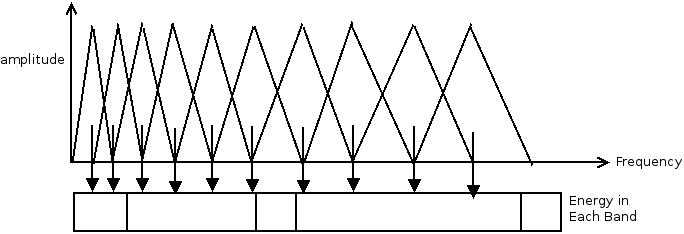
\includegraphics[width=150mm]{resources/melscale}
                        \caption{Mel scale filter bank}
                        \label{fig:Melscale}
                \end{figure}
                This figure shows a set of triangular filters that are used to compute a weights sum of filter spectral components so that the output
                of process approximates to a Mel scale. Each filter's magnitude frequency response is triangular in shape and equal to unity at the
                centre frequency and decrease linearly to zero at centre frequency of two adjacent filters [7,8]. Then, each filter output is the sum of its
                filtered spectral components. After that the following equation is used to compute the Mel for given frequency f in Hz:
                \begin{equation}
                        M(f) = 1125ln\Big(1+\frac{f}{700}\Big)
                \end{equation}
        \item \textbf{Discrete Cosine Transform:}
                This is the process to convert the log Mel spectrum into time domain using Discrete Cosine Transform(DCT). The result of the conversion is
                called Mel Frequency Cepstrum Coefficient. The set of coefficient is called acoustic vectors. Therefore, each input utterance is transformed
                into a sequence of acoustic vector.
\end{enumerate}

\subsubsection{Pitch}
It is a perceptual property of sounds that allows their ordering on a frequency­related scale, or 
more commonly, pitch is the quality that makes it possible to judge sounds as "higher" and "lower" in 
the sense associated with musical melodies.\\  
\\
It is a subjective psychoacoustical attribute of sound, and hence is approximately quantified 
as fundamental frequency.Pitch is an auditory sensation in which a listener assigns musical tones to 
relative positions on a musical scale based primarily on their perception of the frequency of 
vibration.Pitch is closely related to frequency, but the two are not equivalent. Frequency is an 
objective, scientific attribute that can be measured. Pitch is each person's subjective perception  of a 
sound wave, which cannot be directly measured. However, this does not necessarily mean that most 
people won't agree on which notes are higher and lower.\\ 
\\
\textbf{Algorithm}
\begin{enumerate}[(i)]
        \item Model the signal $x_t$ as a periodic function with period T, by definition invariant for a time shift
                of T
                \begin{equation}
                        x_t - x_{t+T} = 0,\hspace{10mm}\forall t
                \end{equation}
                The same is true after taking the square and averaging over a window
                \begin{equation}
                        \sum_{d=t+1}^{t+W}{(x(j)-x(j+\tau))^2} = 0
                \end{equation}
                    Conversely, an unknown period may be found by forming a difference function and searching for 
                    the values of $\tau$ for which the function is zero.
            \item The cumulative mean normalized difference function is calculated by dividing each value of the old 
                    by its average over shorter-lag values. It differs from difference function in the first step in that it 
                    starts at 1 rather than 0, tends to remain large at low lags, and drops below 1 only where the first 
                    difference function falls below average. 
            \item Set an absolute threshold and choose the smallest value of $\tau$ that gives a minimum of the  
                    difference function obtained in the second step deeper than that threshold. If none is found, the 
                    global minimum is chosen instead. With a threshold of 0.1, the error rate drops significantly. 
            \item Each local minimum of the second difference function and its immediate neighbors is fit by a 
                    parabola, and the ordinate of the interpolated minimum is used in the dip-selection process. The 
                    abscissa of the selected minimum then serves as a period estimate. Actually, one finds that the 
                    estimate obtained in this way is slightly biased. To avoid this bias, the abscissa of the corresponding 
                    minimum of the raw difference function(the first) is used instead. 
\end{enumerate}

\subsubsection{Tempo}
The beat is the regularly occurring pattern of rhythmic stresses in music. When we count, tap or clap along 
with music we are experiencing the beat. Try tapping your finger along with different types of music and see 
what happens.\\ 
\\
Tempo is the speed of the beat, usually expressed in Beats Per Minute(BPM). For example, at 120 BPM 
there will be 120 beats in one minute. Tempo can also be expressed verbally with different music terms, 
such as Slowly, Fast, Allegro, or Largo.\\
\\
\textbf{Algorithm}
\begin{enumerate}[(i)]
        \item Parse an audio file into samples, s[n], with a corresponding sampling rate, SR.
        \item Break the audio file into N windows of 1024 samples.
        \item Calculate the FFT of each window.
        \item Calculate the power spectrum(P) of each window form the corresponding FFT results.
        \item Calculate the spectral flux(F) from the power spectrum(P) of each window, i:
                \begin{equation}
                        F_i = (P_i - P_{i-1})^2
                \end{equation}
        \item Find the mean flux, $F_{av}$, across all windows.
        \item Set $F_i$, the flux for each window, to 0 if it is not at least 1.5 times $F_{av}$ (this value
                was experimentally determined). This gives a generous estimation of note onsets.
        \item Use autocorrelation to find the histogram of lag frequencies, L:
                \begin{equation}
                        L[lag] = \sum_{i}^{N}{F[i]F[i+lag]}
                \end{equation}
        \item Calculate the effective sampling rate, $S_{eff}$, found in F and L.
                \begin{equation}
                        SR_{eff} = \frac{SR}{1024}
                \end{equation}
        \item Convert the lag histogram L[lag] into a tempo histogram L[BPM] with bins of beats per
                minute by reversing the order of L and converting the bin lag indices, lag, to BPM:
                \begin{equation}
                        L[BPM] = L\Big(\frac{60*SR_{eff}}{lag}\Big)
                \end{equation}
        \item The result of step (x), L[BPM], is a tempo histogram with bin labels corresponding to beats 
                per minute and bin frequencies correspoding to frequencies of inter-peak intervals.

\end{enumerate}
\subsubsection{Root Mean Square}
The root mean square(abbreviated RMS of rms) is defined as the square root of mean square(the arithmetic mean
of the squares of a set of numbers).
\begin{equation}
        x_{rms} = \sqrt{\frac{1}{n}(x_1^2+x_1^2+...+x_n^2)}
\end{equation}
where there is set of n values \{$x_1, x_2, ......., x_n$\}.

\subsubsection{Spectral Centroid}
The spectral centroid is defined as the center of gravity of the magnitude spectrum of the STFT.
\begin{equation}
        C_t = \frac{\sum\limits_{n=1}^{N}{M_t[n]*n}}{\sum\limits_{n=1}^{N}{M_t[n]}}
\end{equation}
where $M_t[n]$ is the magnitude of the Fourier transform at frame t and frequency bin n.\\
The centroid is a measure of spectral shape and higher centroid values correspond to "brighter" textures with more high frequencies.

\subsubsection{Spectral Flux}
The spectral flux is defined as the squared difference between the normalized magnitudes of successive spectral distributions.
\begin{equation}
        F_t = \sum_{n=1}^{N}{(N_t[n]-N_{t-1}[n])^2}
\end{equation}
where $N_t[n]$ and $N_{t-1}[n]$ are the normalized magnitude of the Fourier transform at the current frame t, and the previous frame t-1, 
respectively.\\ 
The spectral flux is a measure of the amount of local spectral change.

\subsubsection{Spectral Roll-off Point}
The spectral roll-off is defined as the frequency $R_t$ below which 85 per cent of the magnitude distribution is concentrated.
\begin{equation}
        \sum_{n=1}^{R_t}M_t[n] = 0.85*\sum_{n=1}^{N}{M_t[n]}
\end{equation}
The roll-off is another measure of spectral shape.

\subsubsection{Spectral Variability}
  Spectral variability is the standard deviation of the magnitude spectrum. This gives the 
  measure of the variance of a signal's magnitude spectrum. 
  \begin{equation}
          Spectral variability = \sqrt{\frac{1}{N-1}-(\sum_{n=1}^{N}{M[n]-mean})^2}
  \end{equation}
  where M[n] = Magnitude spectrum of the signal at interval n,
  Mean = mean of the magnitude spectrum.

  \subsubsection{Zero Crossing}
The zero crossing is defined as the number of times the waveform changed sign.
\begin{equation}
        Z_t = \frac{1}{2}\sum_{n=1}^{N}{|sign(x[n])-sign(x[n-1])|}
\end{equation}
where the sign fucntion is 1 for positive arguments and 0 for negative arguments and\\
x[n] is the time domain signal for frame t.\\
Time domain zero crossings provide a measure of the noisiness of the signal.



\subsection{Classifier}
In machine learning and statistics, classification is the problem of identifying to which of a set of categories(sub-populations) a 
new observation belongs, on the basis of a training set of data containing observations(or instances) whose category membership is known.
In the terminology of machine learning, classification is considered an instance of supervised learning where a training set of correctly identified observations is available.
The corresponding unsupervised procedure is known as clustering, and involves grouping data into categories based on some measure of inherent similarity or distance.
An algorithm that implements classification,especially in a concrete implementation, is known as a classifier.\\
\\
A variety of methods have been used for music classification. Some of the popular ones are
SVM, K-means, K-nearest neighbours and variants of Neural Networks.
The results are also widely different. In \cite{Neumayer2004} 61 per cent accuracy has been achieved using
a Multilayer Perceptron based approach while in \cite{Kour2015}, the authors have managed 95 per cent
(for Back Propagation Neural Network) and 83 per cent (for SVM).
In \cite{Koerich2013}, the authors have achieved 71 per cent accuracy using an additional rejection and
verification stage.\\
\\
In \cite{Haggblade2011}, simpler and more naive approaches (k-NN and k-Means); and more sophisticated
neural networks and SVMs have been compared. The author found the latter gave better
performance.\\
\\
However, lots of unique methods – either completely novel or a variation of a standard
method – have been put into use too. In \cite{Nasridinov2014}, the authors propose a method that uses Chord
labeling (ones and zeros) in conjunction with a k-windowSubsequenceMatching algorithm
used to find subsequence in music sequence and a Decision tree for the actual genre classifi-
cation.\\
\\
It is also noted that high-level and contextual concepts can be as important as low-level
content descriptors\cite{Anglade2010}.\\
\\
After these all research, we decided to go with K-means, artificial neural network based on backpropagation
and support vector machine. Artificial neural network and support vector machine were chosen as they appeared to be famous in the field. Our choice for K-means 
was based on the fact that it was simple yet powerful unsupervised procedure.

\subsubsection{K-means Clustering}

K-means is one of the most popular algorithm used for clustering of a given data sets. It is a method of vector quantization, originally
from signal processing, that is popular for cluster analysis in data mining. It aims at partition n obsevations into k clusters in which each observation
belongs to the cluster with the nearest mean, serving as a prototype of the cluster. This results in a partitioning of the data space into Voronoi cells. 
In other words, it clusters all the data points which resemble close
to each other or we can that it cluster all those data points together which have the lowest cost among themselves based on the distance metric.
The problem is computationally difficult(NP-hard); however, there are efficient heuristic algorithms that are commonly employed and converge quickly to a local optimum.
It has loose relationship to the k-nearest neighbor classifier.\\ 
\\
Regarding computational complexity, finding the optimal solution to the k-means clustering problem for obsevations in d dimensions is NP-hard in genral Euclidean space
d even for 2 clusters and NP-hard for a general number of clusters k even in the plane. It k and d (the dimension) are fixed, the problem can be solved in time
$O(n^{dk+1}logn)$, where n is the number of entities to be clustered.
The choice for this algorithm was based on our research and some had already implemented it \cite{Haggblade2011}. Most of the research papers has enlisted this algorithm like in \cite{muller2011}, 
\cite{Hamerly2002}, \cite{Haggblade2011}. So, our reason for implementation of this algorithm was:
\begin{enumerate}[(i)]
        \item Most of the research papers has shown its use in music classification.
        \item It is a pretty straightforward and simple algorithm.
        \item We wanted to have full control over all aspects related to the implementation: the initialization method, distance metric, etc.
\end{enumerate}
The implementation however is basic in the sense that no modification has been done on the algorithm to better suit the problem domain. 
Some finer points of the implementation are discussed below after quickly going over the algorithm itself.\\ 
\\
\textbf{Algorithm}\\
Let X = { $x_1, x_2,.... ,x_n$ be the set of data points and V = { $v_1,v_2 , ...,v_c$ } be the set of centers. 
        \begin{enumerate}[(i)]
                \item Randomly select 'c' cluster centers. 
                \item Calculate the distance between each data point and cluster centers. 
                \item Assign the data point to the cluster center whose distance from the cluster center is minimum of all the cluster centers. 
                \item Recalculate the new cluster center: 
                        \begin{equation}
                                v_i=\frac{1}{c_i}\sum_{j=1}^{c_i}{x_i}
                        \end{equation}
                \item  Recalculate the distance between each data point and new obtained cluster centers. 
                \item If no data point was reassigned then stop, otherwise repeat from step 3).
        \end{enumerate}
\textbf{Initialization method}\\
Commonly used initialization methods are Forgy and Random Partition. The Forgy method randomly chooses k observations from the data set and uses
these as the initial means. The Random Partition method first randomly assigns a cluster to each observation and then proceeds to the update step, thus
computing the initial mean to be the centroid of the cluster’s randomly assigned points. The Forgy method tends to spread the initial means out, while
Random Partition places all of them close to the center of the data set. According to \cite{Kour2015}, the Random Partition method is generally preferable for
algorithms such as the k-harmonic means and fuzzy k-means. For expectation maximization and standard k-means algorithms, the Forgy method of initialization is preferable.\\
\\
And with these facts in mind, we went for the random initialization method. This method has been used in \cite{muller2011} too although they have also added
the constraint that the centroids be separated by at least a threshold KL-divergence distance. As the choice of initial centroids have a drastic
effect on the cluster formed, we have also considered other methods of initialization such as the breakup method which uses the actual data points
and the scrambled midpoints method which uses synthetic data points as suggested in \cite{prasad2007}. So after our research on this, we found that 
scrambled midpoints to be much more efficient and lead to better clustering. So based on \cite{Apon2006}, scrambled midpoints technique was
chosen for initialization.\\
\\ 
In scrambled midpoints initialization method, at first our whole data range or in our case each feature range was broken down into k-paritions which were
all equal. Then midpoints were taken of those equal partitions for each feature partition range. Povided there are n-features with k
number of clusters needed, then we have n*k different possibilities. Now all these midpoints of each range of n-features were scrambled among
each other to form k different initialization points/vectors representing all those n-features. It should be clear that there is no repetition of the midpoint of same range 
of same feature during scrambling of midpoints to form initialization points/vectors.\\  
\\
\textbf{Distance Metric}\\
Apart from the initialization method, K-means is also highly sensitive to the distance metric used. There are many distance metric but most popular ones are: 
\begin{itemize}
        \item Manhattan distance
        \item Euclidean distance
        \item Minkowski distance
\end{itemize}
Most of the times, K-Means is implicitly based on pairwise Euclidean distances between points, because the sum of squared deviations from centroid (that it tries to minimize) is equal
to the sum of pairwise squared Euclidean distances divided by the number of points \cite{Neumayer2004}.\\ 
\\
As such, we decided to use Euclidean distance with weights for the three different features added to give us a way to control the metric. Thus, the
distance between two songs S1 and S2 is given by: 
\begin{equation}
        Distance(d)=\sqrt[2]{w_I(I_1-I_2)^2+w_M\sum_{i}{(M_{1i}-M_{2i})^2}+w_R\sum_{i}{(R_{1j}-R_{2j})^2}}
\end{equation}
Where: $w_I$ , $w_M$  and $w_R$ are the weights for Intensity, MFCC and Rhythm respectively. 

\subsubsection{Artificial Neural Network}
In machine learning and cognitive science, an artificial neural networks(ANN) is a network inspired by biological neural networks(the central nervous systems of 
animals, in particular the brain) which are used to estimate or approxiamte functions that can depend on a large numbers of inputs that are generally unknown.
Our research shows whether the research is related to our field or other, most of the time for machine learning researchers used artificial neural network.
So our choice was simple as it was based on supervised learning and comparatively simple than other complicated unsupervised learning.
Research papers \cite{Koerich2013}, \cite{Neumayer2004}, ,\cite{Anglade2010}, \cite{Haggblade2011} and \cite{Kour2015} shows the implementation of artificial neural network in the field of
music classification.\\
\\
Artificial neural networks are typically specified using three things:
\begin{itemize}
        \item \textbf{Architecture:} 
                It specifies what variables are involved in the network and their topological relationships- for example the variable involved
                in a neural network might be the weights of the connections between the neurons, along with activities of the neurons. In an artificial
                neural network, there are one or more hidden layers in between input and output layers with all the neurons connecting to each other.
        \item \textbf{Activity Rule:}
                Most neural network models have short tiem-scale dynamic: local rules define how the activities of the neurons change in reponse to each other.
                Typically the activity rule depends on the weights(the parameters) in the network.Here in our case, the set of input neuronse
                is activated by the feature values like MFCC, pitch,etc. There activation function present to trigger the respective neuron. Most of the time
                activation function are non linear, differential mathematical functions like sigmoid, hyperbolic tangent, etc.
        \item \textbf{Learning Rule:}
                The learning rule specifies the way in which the neural network's weights change with time as the learning takes progress. This learning is usually viewed as 
                taking place on a longer time place than time scale of the dynamicx under the activity rule. Usually the learning rule will depend on the activites of the 
                neurons. In our case the learning depends on the values of the target values supplied by a teacher and on the current value of the weights.
\end{itemize}

For a system, generally the architecture is created as per the need. Generally for that there is lot of trial and error methodology involved
to determine the correct number of hidden layers and neurons needed. In most cases, one hidden layer is suffiecient for the system but if 
the nature of system or data is perplexing then in accordance to expected result and current behavior, number of hidden layers of nodes can be increased.\\
\\
The concept of cost function is an important in context of artificial neural network. It measures how far away a particular solution is from an
optimal solution. We can also say that the cost of the optimal solution is minimum. So, the target of our artifical neural network is to
try to meet the cost of optimal solution. While it is possible to define some arbitrary ad hoc cost fucntion, frequently a particular cost will be used, either
because it has desirable properties (such as convexity) or because it arises naturally from a particular formulation of problem. Ultimately, the cost
fucntion will depend on the desired task. One of the mostly used cost function is squared error measure between the output value O and the target value t.
\begin{equation}
        E = (t-y)^2
\end{equation}
where E is the discrepancy or error.\\
\\
Using this cost, the neural network tries to adjust it weights in order to minimize the cost function. This exact process is called learning.
Supervised learning, unsupervised learning and reinforcement learning are the three major paradigms of learning. We are opting for the supervised learning.
The reason for this choice is that unsupervised learning and reinforcement learning are comparatively more complex and also supervised learning have been doing 
great job in this music classification field based on research papers \cite{Neumayer2004}, \cite{Haggblade2011}, \cite{Kour2015}. Supervised learning 
requires the correct class label to be provided along with the training dataset for the neural network so that it can adjust it's weight based on the cost function 
of incorrect/correct class prediction. Backpropagation algorithm is the most popular learning algorithm for neural network out there. The reason for
its popularity might be its simplicity in terms of concept and wide applicability. It's also based on supervised learning. When one tries to minimize cost function
using gradient descent for the class of neural networks called multilayer perceptrons(MLP), one obtains the common and well-known backpropagation algorithm for training neural networks.\\
\\
Backpropagation is a common method of training artificial neural networks used in conjunction with an optimization method such as gradient descent. The 
method calculates the gradient of a loss function with respect to all the weights in the network. The gradient is fed to the optimization method wihich in turn uses it to
update the weights, in an attempt to minimize the loss function. It is a generalization of delta rule to multi-layered feedforward networks, made possible
by using the chain rule to iteratively compute gradients for each layer. Requirements of backpropagation mehod are:
\begin{itemize}
        \item It requires a known, desired output for each input value in order to calculate the loss function gradient.
        \item It requires the activation function used by the artificial neurons/nodes to be differentiable.
\end{itemize}
\textbf{Algorithm}
\begin{enumerate}[(i)]
        \item Run the network forward with your input data to get the network output.
        \item For each output node compute
                \begin{equation}
                        \delta_k = O_k(1 - O_k)(O_k - t_k)
                \end{equation}
        \item For each hidden node calculate
                \begin{equation}
                        \delta_j = O_k(1 - O_k) \sum_{k \in K}{\delta_kW_{jk}}
                \end{equation}
        \item Update the weights and biases as follows:\\
                Given
                \begin{equation}
                        W = -\eta \delta_l O_{l-1}
                \end{equation}
                \begin{equation}
                        \Delta \theta = -\eta \delta_l
                \end{equation}
                apply
                \begin{equation}
                        W + \Delta W \to W
                \end{equation}
                \begin{equation}
                        \theta + \Delta\theta \to \theta
                \end{equation}
\end{enumerate}
where i, j and k represents the input layer, hidden layer and ouput layer respectively,\\
O is the output of a neuron/node,\\
t is the target value,\\
K is the total number of output neurons/nodes,\\
$\Delta$ represent the difference,\\
l denotes every layer.\\
\\
$\eta$ is the learning rate which is defined as the ratio(percentage) that influences the speed and quality of learning.The greater the ratio, the faster the neuron trains;
the lower the ratio, the more accurate the training is. $\theta$ is the bias term which is involved in adjusting the shifting of activation function. The sign of the gradient
of a weight indicates where the error is increasing, this is why the weight must be updated in the opposite direction. The algorithm above is
repeated until performance of the network is satisfactory.

\subsubsection{Support Vector Machine}

In machine learning, support vector machines (SVM) are supervised learning models with 
associated learning algorithms that analyze data used for classification analysis.They are new statistical learning technique that can be seen as a new method for training
classifiers based on polynomial functions, radial basis functions, neural networks, splines or other functions. The popularity of Support Vector machine is huge as lot of researcher papers
\cite{Koerich2013}, \cite{Anglade2010}, \cite{Haggblade2011}, \cite{Kour2015} shows its implementation. Not only in the field of music classification but also on various artificial intelligence field like handwriting
recognition, biological and other sciences. It was also able to overthrow general neural network until the advent of deep learning.\\
\\
The basic support vector machine (SVM) is a binary linear classifier which chooses the hyperplane that represents the largest separation, or margin, between the two classes. So  Support vector machines use
a hyperplane to create a classifier. If such a hyperplane exists, it is known as the maximum­margin hyperplane and the linear classifier it defines is known as a maximum margin classifier. 
If there exists no hyperplane that can perfectly split the positive and negative instances, the soft 
margin method will choose a hyperplane that splits the instances as cleanly as possible, while still 
maximizing the distance to the nearest cleanly split instances. For problems that cannot be linearly separated in the input space, this machine offers a possibility to find a solution by making 
a non-linear transformation of the original input space into a high dimension feature space where an optimal separating hyper plane can be found. Those separating planes are optimal, which means
that a maximal margin classifier with respect to the training data set can be obtained. It is developed by Vladimir Vapnik and co-workers at AT\&T Bell Laboratories in 1995.\\
\\
The nonlinear SVMs are created by applying the kernel trick to maximum­margin hyperplanes. 
The resulting algorithm is formally similar, except that every dot product is replaced by a nonlinear kernel 
function.\\
\\
\textbf{Kernel Function}\\
The simplest way to divide two groups is with a straight line, flat plane or an N-dimensional hyper plane.
But what if the points are separated by a non-linear region. In such case we would need a non-linear dividing line. Rather than fitting
non-linear curves to the data, support vector machine handles this by using a kernel function to map the data into a different space where
a hyperplane can be used to do the separation. \cite{Anglade2010} shows the use of second order polynomial kernel in the support vector machine.
So, kernel function allows the algorithm to fit the maximum­margin hyperplane in a transformed
feature space. The transformation may be nonlinear and the transformed space be high dimensional. For example, the 
feature space corresponding to Gaussian kernel is a Hilbert space of infinite dimension. Thus though the 
classifier is a hyperplane in the high dimensional feature space, it may be nonlinear in the original input 
space. Maximum margin classifiers are well regularized, so the infinite dimension does not spoil the 
result as the separation will be performed even with very complex boundaries.\\
\\
The effectiveness of SVM depends on the selection of kernel, the kernel’s parameters, and soft 
margin parameter c. Given a kernel, best combination of c and kernel’s parameters is often selected by a 
grid­search with cross validation. 
The dominant approach for creating multiclass SVMs is to reduce multi­class problem into 
multiple binary classification problems. Common methods for such reduction is to build binary classifiers 
which distinguish between (i) one of the labels to the rest (one­versus­all) or (ii) between every pair of 
classes (one­versus­one). Classification of new instances for one­versus­all case is done by a 
winner­takes­all strategy, in which the classifier with the highest output function assigns the class. For the 
one ­versus­one approach, classification is done by a max­wins voting strategy, in which every classifier 
assigns the instance to one of the two classes, then the vote for the assigned class is increased by one vote, 
and finally the class with most votes determines the instance classification. To tackle the same multiclass problem \cite{Haggblade2011} has the  
utilization of DAG(Directed Acyclic Graph) SVMs in which a directed acyclic graph(DAG) of two-class SVMs is trained on each pair of classes in the data set.

\subsection{Testing and Validation}
While building a software product, the concept of testing and validation plays an important role throughout its development.
Along with the development of a software product, numerous testing and validation are need to be performed regulary.
In fact, most of the development period is given to testing and validation. It's important as it conforms to whether we are building
product right and whether we are building the right product. After series of testing and validation only we can point that the system
conforms to the desired specifications and need.\\
\\
Since our software project is also research oriented, so we need series of rigorous testing. Not only this, being a predictive system/model
a type of validation and measure for performance is a must, so that it can analyze the result and decide how to progress further accounting the fact.
For our system, we chose cross-validation after we confronted it's popularity for a predictive model and ease of use. Similarly for measure of performance we chose recall, presicion 
and F-measure.\\

\subsubsection{Cross-validation}
Cross-validation is a technique for estimating the performance of a predictive model.
Cross-validation, sometimes called rotation estimation is a model validation technique for assessing how the
results of a statistical analysis will generalize to an independent data set. In a predictive problem like our project, a model is usually given a dataset of known data(training dataset) on which 
the model is trained, and a dataset of unknown data (or first seen data) against which the model is tested (testing dataset). The goal of cross validation is to define a dataset
to "test" the model in the training phase(validation dataset), in order to limit problems like overfitting, give an insight on how the model will generalize to an independent dataset(and unknown dataset, for instance from 
a real problem),etc.\\
\\
One of the main reasons for using cross-validation instead of using the conventional validation is that there is not enough data available to partition it into separate training and test sets without losing
significant modelling or testing capability. There are several cross-validation method out there like leave-p-out cross-validation, leave-one-out cross validation,2-fold cross validaiton, repeated random 
sub-sampling validation, etc. But we decide to got with k-fold cross validation. The main reason for this selection is that k-fold cross-validation estimator can prove to have a lower variance than a single hold-out set 
estimator if the amount of data available is limited. Our main goal with k-fold cross validation is to estimate the expected level of fit of a model to a dataset that is independent of the data that were
used to train the model.\\
\\
In k-fold cross-validation, the original sample is randomly partitioned into k equal sized subsamples. Of the k subsamples,
a single subsample is retained as the validation data for testing the model, and the remaining k − 1 subsamples are used as training
data. The cross-validation process is then repeated k times (the folds), with each of the k subsamples used exactly once as the validation data. The k results from the
folds can then be averaged to produce a single estimation. The advantage of this method over repeated random sub-sampling (see below) is that all
observations are used for both training and validation, and each observation is used for validation exactly once. ten-fold cross-validation is currently
applied in our system. Our music data set is first divided into ten equal samples of songs, and on every run for ten times, a different sample of songs are used for
testing and the rest for training.\\
\\
This k-fold validation validation process is applied with each performance metrics and the appropriate features are taken to classify in our system.

\subsubsection{Measure of Performance}
In a predictive problem, we always need a measure of performance for that predictive model along with cross validation. Based on the value of different attributes falling under 
the measure of performance, we can then have the knowledge of how well the system is performing. It is important because as a matter of fact it provides much deeper insight of the performance of
the predictive model, not only accuracy.\\
\\
Our measure of performance include precision, recall and F-measure. We can say our measure of performance are based on the relevant and non-relevent documents. In this case,
relevant documents are those one which simply belong to the relevant category. Relevant category is also called the true positives. True positive is the number of items correctly
labeled as belong to the positive class or say which are predicted correctly. The not relevant documents are those one which simply are not relevant to the category or say they are false negative. 
False negative is the number of negative items which are predicted to fall under the positive class. False Positive is the number of negative items which are predicted to be in true class.
Similarly, true negative is the number of negative items which are correctly predicted to fall under negative class.

\begin{itemize}
        \item \textbf{Precision}\\
                The precision of a measurement system, related to reproducibility and repeatability, is the degree to which repeated measurements under unchanged
                conditions show the same results. In a classification task, the precision for a class is the number of true positives divided by the total number of elements labeled as 
                belonging to the positive class. A perfect precision score of 1.0 means that every result retrieved by a search was relevant which means falling to the specified class.
                But precision does not say whether all items of that class were correctly predicted.
                \begin{equation}
                        Precision = \frac{True Positive}{True Positive + False Positive}
                \end{equation}
        \item \textbf{Recall}\\
                Recall literally is how many of the true positives were recalled (found), i.e. how many of the correct hits were also found. Recall is also sometimes called sensitivity or probability of detection.
                It is the true positive rate as it measure the proportion of positives that are correctly identified as such. Recall is the number of true positives divided by the total number of elements
                that actually belong to the positive class. A perfect recall score of 1.0 means that all relevant documents were retrieved by search. We can also say that perfect recall shows that all items of a
                class were labeled fall under same class. But recall does not say that how many other items were misclassified to fall under same class.
                \begin{equation}
                        Recall = \frac{True Positive}{True Positive + False Negative}
                \end{equation}
        \item \textbf{F measure}
               A measure that combines precision and recall is the harmonic mean of precision and recall. 
                F measure is the weighted harmonic mean of its the precision and recall of a system. It is sometimes called as balanced F-score. This measure is approximately the average of the two when they are close, and is more generally
                the harmonic mean which for the case of two numbers coincides with the square of the geometric mean divided by the arithmetic mean. There are several reasons that the F-score can be criticized in particular 
                circumstances due to its bias as an evaluation metric. This is also known as the $F_1$ measure, because recall and precision are evenly weighted.
                \begin{equation}
                        F = 2*\frac{Precision*Recall}{Precision+Recall}
                \end{equation}
        \end{itemize}
        All three performance metrics have been used to determine the best features to be used for classification in cases of genre, arousal and valence.\\ 
        \\
    As depicted in the result and analysis section, we can see that not all the features are suitable for the classification. Some features such as intensity or pitch do not contribute 
    the classification but some features such as Mel Frequency Coefficients(MFCC) contribute greatly to the classifier’s performance. 




\newpage
\section{SYSTEM ANALYSIS}
\subsection{Requirement Specification}
\subsubsection{High Level Requirements}
As our system is a music classification system, so we need our system to classify any given music file among the following genre and mood.
Genres include:
    \begin{itemize}
    \item Hip-hop
    \item Rock
    \item Jazz
    \item Classical
    \item Pop
    \end{itemize}
Mood include:
    \begin{itemize}
    \item Depressive
    \item Frantic
    \item Exuberant
    \item Contentment
    \end{itemize}
    The classification of the audio files based on genre and mood can be then be used in the creation of auto generated playlists.After each high level requirements are identified, corresponding intermediate level requirements
    (ILRs) are also identified. These list the feature metadata used to classify the audio.
\subsubsection{Functional Requirements}
\begin{itemize}
        \item The system shall classify among the given genre and mood. Mood is classified in terms of arousal and valence. 
        \item The system shall work on various music file format like mp3, wav, etc.
        \end{itemize}

\subsubsection{Non-Functional Requirements}
Non­functional requirement is a requirement that specifies criteria that can be used to judge the 
operation of a system, rather than specific behaviors.\\ 
\\
The non­functional requirement in our project are: 
\begin{itemize}
        \item Code Documentation
        \item Project Documentation
        \item Code Quality
        \item Performance
        \item Fault Tolerance
        \item Scalability
        \item Testability
        \item Maintainability
        \end{itemize}
                
\subsection{Feasibility Assessment}
A feasibility assessment or feasibility analysis is a preliminary study undertaken before the real work of a project starts to ascertain the likelihood fo the project's success.
It is an analysis of possible alternative solutions to a problem and a recommendation on the best alternative. It, for example, can decide whether an order processing be carried out by a new system more 
efficiently than the previous one. It can be thought as an assessment of the practicality of a proposed project.\\
\\
A feasibility study aims to objectively and rationally uncover the strengths and weakness of an existing project paradigm, opportunities and threats present in the environment, the resources required to carry through, and ultimately the prospects
of success. In simplest terms, the two criteria to judge feasibility are cost required and value to be attained. A well-designed feasibility study should provide a historical background of the project,
a description of the project and details of operations and technicality needed.Generally feasibility studies always precede technical development and project implementation. A feasibility study evaluates the project's potential for success. It must there be
conducted with an objective, unbiased approach to provide information upon which decisions can be based.\\
\\
The acronym TELOS refer to the five areas of feasibility:
\begin{itemize}
        \item Technical feasibility
        \item Economic feasibility
        \item Legal feasibility
        \item Operational feasibility
        \item Scheduling feasibility
\end{itemize}

\subsubsection{Technical Feasibility}
After our thorough research we decided to go with the features mentioned above. We also chose simple but powerful algorithm to do the classification.
Since our first priority is to do all the coding from the scratch, we do not guarantee to be optimised at highest level in terms of space and time complexity as we lack such expertise and experience of a professional developer.
Since there is no standard procedure to check the accuracy of the extracted features, we might have hard time in validating the feature extraction process.
But based on our experience we can do most of the coding by ourselves or at least try and then analyze the result. If we find any difficulty in future then we can use existing library like TarsoDSP,MP3SPI, etc. which are proved to provided excellent audio processing.

\subsubsection{Economic feasibility}
Being a research oriented project, our focus is soley based on knowledge and not on any monetary factors at all.
Since our project is just the beginning portion which could be a huge leading factor in future and bring
revolution in music industry, our current product might not be able to provide that much of montary benefit but sure it will be contributing to a huge research ahead in future.
It's wide variety of application is sure to provide huge amount of benefits in future.
Then, talking about the cost, as no hardware is required in our project so we can say there is almost no loss involved in monetary terms. Hence implementation can be started.

\subsubsection{Operational Feasibility}
Our system is not a hardware based. A computer is enough for it to run. We can say that there is no extra need for any hardware. Since we will be doing digital signal processing for the first we will be going to need
the knowledge of signal processing.

\subsubsection{Schedule feasibility}
Our system is not that huge or complex. Therefore it will be easy to follow the pre-planned schedule for development. But however given our novice nature, we might lag a little behind the schedule provided a complex bug in our system arises.

\subsubsection{Legal feasibility}
Legal feasibility determines whether the proposed system conflicts with legal requirements.
All of the algorithms does not have any copyright attached with them. We found that our conflicting factor might only be on the use of the database provided provided we misuse it or violate some conditions or if 
we illegally download it.




\newpage
\section{SYSTEM DESIGN}



\newpage
\section{SYSTEM DEVELOPMENT}


\newpage
\section{RESULTS AND ANALYSIS}


\subsection{Dataset pre-processing}

\subsubsection{Genre Dataset}
In \cite{Downie2003}, Downie presents the problem of a lack of a proper baseline dataset for the AMGC problem, which meant research teams couldn’t scientifically compare and contrast their different approaches.\\
\\
However, the publicly available GTZAN dataset introduced in \cite{Tzanetakis2002}, solved most parts of the issue by soon becoming the standard dataset used by researchers across the world. We too used this dataset for this project. The dataset contains 100 representative excerpts from ten different genre. They were taken from radio, compact disk, and MP3 compressed audio files. All the files are stored as 22 050 Hz, 16-bit, mono audio files. The Genres dataset has the following classes: classical, country, disco, hiphop, jazz, rock, blues, reggae, pop, metal. Among them we were only concerned with five genre as mentioned in Chapter 1: classical, hiphop, jazz, rock, and pop, So, we had a total of 500 songs in our dataset.

\subsubsection{Mood Dataset}
Due to the high variability in the emotional models adopted (whether categorical or dimensional), there have been no popular baseline dataset for MER task.\\
\\
So, to tackle the issue, in 2013, Soleymani et al. \cite{Soleymani2013} created a 1000 songs dataset for emotional analysis of music which uses the Valence-Arousal axes for representing emotional values for songs.\\
\\
The songs, in the dataset, each 45 seconds long, were collected from FMA. They used Amazon Mechanical Turk as a crowdsourcing platform for collecting more than 20,000 annotations on the 1,000 songs.\\
\\
Furthermore, their analysis on the annotations revealed a higher agreement in arousal ratings compared to the valence ratings.\\
\\
We have used a filtered version (with some redundancies removed) of that dataset resulting in a final set of 744 songs. We further labeled them as high/low arousal and high/low valence songs based on the numerical values in the dataset. To achieve equal number of songs in each class, we finally used 600 songs of those 744 songs. 

\subsection{Testing and Validation}
While building a software product, the concept of testing and validation plays an important role throughout its development.
Along with the development of a software product, numerous testing and validation are need to be performed regulary.
In fact, most of the development period is given to testing and validation. It's important as it conforms to whether we are building
product right and whether we are building the right product. After series of testing and validation only we can point that the system
conforms to the desired specifications and need.\\
\\
Since our software project is also research oriented, so we need series of rigorous testing. Not only this, being a predictive system/model
a type of validation and measure for performance is a must, so that it can analyze the result and decide how to progress further accounting the fact.
For our system, we chose cross-validation after we confronted it's popularity for a predictive model and ease of use. Similarly for measure of performance we chose recall, presicion 
and F-measure.\\

\subsubsection{Cross-validation}
Cross-validation is a technique for estimating the performance of a predictive model.
Cross-validation, sometimes called rotation estimation is a model validation technique for assessing how the
results of a statistical analysis will generalize to an independent data set. In a predictive problem like our project, a model is usually given a dataset of known data(training dataset) on which 
the model is trained, and a dataset of unknown data (or first seen data) against which the model is tested (testing dataset). The goal of cross validation is to define a dataset
to "test" the model in the training phase(validation dataset), in order to limit problems like overfitting, give an insight on how the model will generalize to an independent dataset(and unknown dataset, for instance from 
a real problem),etc.\\
\\
One of the main reasons for using cross-validation instead of using the conventional validation is that there is not enough data available to partition it into separate training and test sets without losing
significant modelling or testing capability. There are several cross-validation method out there like leave-p-out cross-validation, leave-one-out cross validation,2-fold cross validaiton, repeated random 
sub-sampling validation, etc. But we decide to got with k-fold cross validation. The main reason for this selection is that k-fold cross-validation estimator can prove to have a lower variance than a single hold-out set 
estimator if the amount of data available is limited. Our main goal with k-fold cross validation is to estimate the expected level of fit of a model to a dataset that is independent of the data that were
used to train the model.\\
\\
In k-fold cross-validation, the original sample is randomly partitioned into k equal sized subsamples. Of the k subsamples,
a single subsample is retained as the validation data for testing the model, and the remaining k - 1 subsamples are used as training
data. The cross-validation process is then repeated k times (the folds), with each of the k subsamples used exactly once as the validation data. The k results from the
folds can then be averaged to produce a single estimation. The advantage of this method over repeated random sub-sampling (see below) is that all
observations are used for both training and validation, and each observation is used for validation exactly once. ten-fold cross-validation is currently
applied in our system. Our music data set is first divided into ten equal samples of songs, and on every run for ten times, a different sample of songs are used for
testing and the rest for training.\\
\\
This k-fold validation validation process is applied with each performance metrics and the appropriate features are taken to classify in our system.

\subsubsection{Measure of Performance}
In a predictive problem, we always need a measure of performance for that predictive model along with cross validation. Based on the value of different attributes falling under 
the measure of performance, we can then have the knowledge of how well the system is performing. It is important because as a matter of fact it provides much deeper insight of the performance of
the predictive model, not only accuracy.\\
\\
Our measure of performance include precision, recall and F-measure. We can say our measure of performance are based on the relevant and non-relevent documents. In this case,
relevant documents are those one which simply belong to the relevant category. Relevant category is also called the true positives. True positive is the number of items correctly
labeled as belong to the positive class or say which are predicted correctly. The not relevant documents are those one which simply are not relevant to the category or say they are false negative. 
False negative is the number of negative items which are predicted to fall under the positive class. False Positive is the number of negative items which are predicted to be in true class.
Similarly, true negative is the number of negative items which are correctly predicted to fall under negative class.

\begin{itemize}
        \item \textbf{Precision}\\
                The precision of a measurement system, related to reproducibility and repeatability, is the degree to which repeated measurements under unchanged
                conditions show the same results. In a classification task, the precision for a class is the number of true positives divided by the total number of elements labeled as 
                belonging to the positive class. A perfect precision score of 1.0 means that every result retrieved by a search was relevant which means falling to the specified class.
                But precision does not say whether all items of that class were correctly predicted.
                \begin{equation}
                        Precision = \frac{True Positive}{True Positive + False Positive}
                \end{equation}
        \item \textbf{Recall}\\
                Recall literally is how many of the true positives were recalled (found), i.e. how many of the correct hits were also found. Recall is also sometimes called sensitivity or probability of detection.
                It is the true positive rate as it measure the proportion of positives that are correctly identified as such. Recall is the number of true positives divided by the total number of elements
                that actually belong to the positive class. A perfect recall score of 1.0 means that all relevant documents were retrieved by search. We can also say that perfect recall shows that all items of a
                class were labeled fall under same class. But recall does not say that how many other items were misclassified to fall under same class.
                \begin{equation}
                        Recall = \frac{True Positive}{True Positive + False Negative}
                \end{equation}
        \item \textbf{F measure}
               A measure that combines precision and recall is the harmonic mean of precision and recall. 
                F measure is the weighted harmonic mean of its the precision and recall of a system. It is sometimes called as balanced F-score. This measure is approximately the average of the two when they are close, and is more generally
                the harmonic mean which for the case of two numbers coincides with the square of the geometric mean divided by the arithmetic mean. There are several reasons that the F-score can be criticized in particular 
                circumstances due to its bias as an evaluation metric. This is also known as the $F_1$ measure, because recall and precision are evenly weighted.
                \begin{equation}
                        F = 2*\frac{Precision*Recall}{Precision+Recall}
                \end{equation}
        \end{itemize}
        All three performance metrics have been used to determine the best features to be used for classification in cases of genre, arousal and valence.

\subsection{Audio Pre-processing}
\subsubsection{Effect of Window Functions}
We tried out five window functions to smoothen the data frames obtained from the samples. 

\begin{figure}[h!]
        \centering
        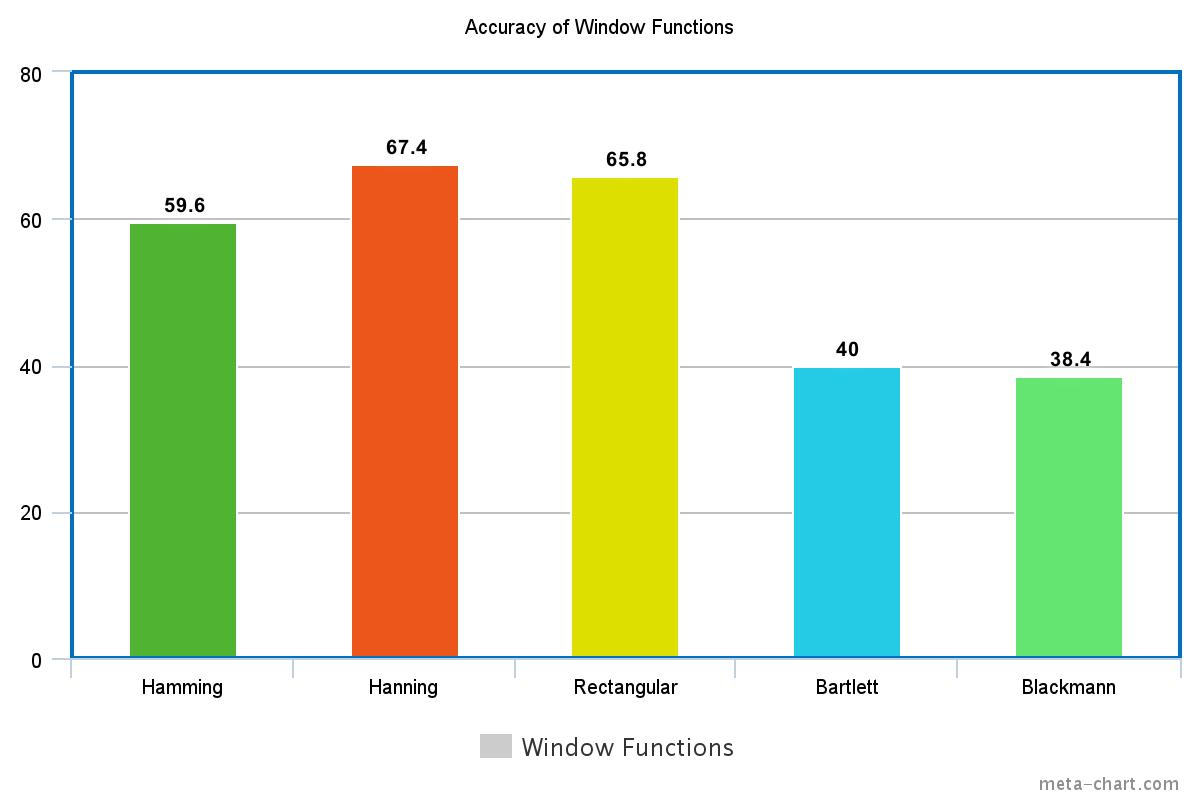
\includegraphics[width=130mm]{resources/mehang/6.3/window}
        \caption{Effect of window functions}
\end{figure}

As seen from the figure, Hanning window gave the best performance. 

\subsubsection{Effect of Frame Size}
The Frame-size needs to be small enough to be statistically invariant but big enough to capture sufficient information. Generally, 20-40ms is taken as the frame size. We tested the frame size according to the number of samples per frame: 512, 1024, 1536 and 2048 samples which correspond to roughly 11.5ms, 23ms, 34.5ms and 46 ms for our songs which have a sampling rate of 44.1 KHz.

\begin{figure}[h!]
        \centering
        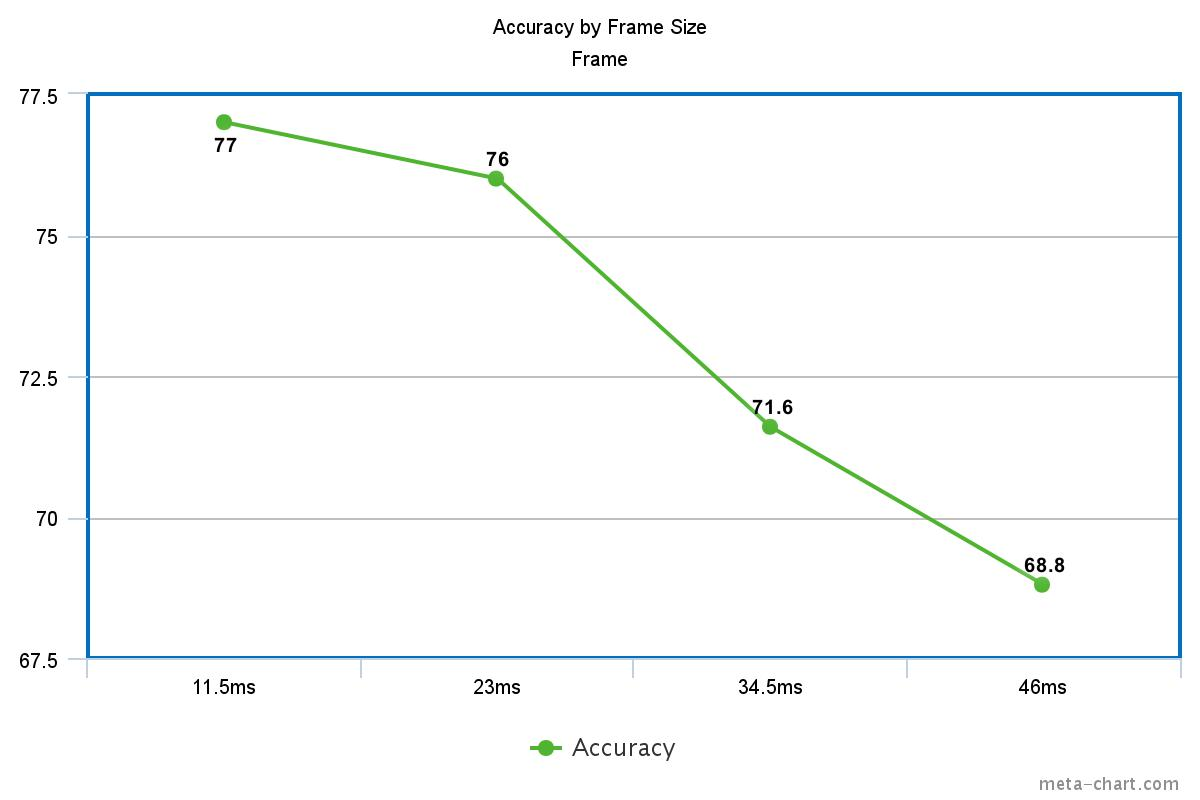
\includegraphics[width=170mm]{resources/mehang/6.3/Frame}
        \caption{Effect of frame size}
\end{figure}

As seen in the figure, frame size of 11.5ms and 23ms performed considerably better than the bigger frame sizes. We chose the 23ms (1024 samples) frame size because the smaller 512 sample frame size would lead to higher number of frames and hence necessitate more computation.

\subsubsection{Effect of Frame Overlap}
We explored four different overlapping schemes: zero per cent, 25 per cent, 50 per cent and 75 per cent overlap.\\
\\
In each of the cases, we received almost the same accuracy (75.4 per cent on No-overlap, 75.8 per cent on Quarter overlap, 76 per cent on half-overlap, and 75.2 per cent on three-quarters overlap). And so, as it seemed to indicate that the overlapping didn’t have any bearing on our results, we chose the less computationally intensive option of using no overlap at all. 

\subsubsection{Effect of Pre-Emphasis}
Pre-emphasis decreased the accuracy from 75.4 per cent to 62.6 per cent.

\newpage
\subsection{Analysis of Features}
\subsubsection{Genre Based Classification}
\begin{table}[h!]
        \caption{Genre classification using ANN}
        \begin{center}
                \begin{tabular}{|l|l|l|l|l|l|l|}
                        \hline Feature & Classical & Hiphop & Jazz & Pop & Rock & Overall\\
                        \hline Spectral Centroid & 47.54 & 11.92 & 11.61 & 51.25 & 18.89 & 28.40\\ 
                        \hline MFCC & 92.45 & 83.42 & 91.57 & 82.98 & 74.44 & 84.20 \\
                        \hline Zero Crossing & 63.29 & 48.31 & 39.83 & 52.65 & 52.00 & 51.20\\
                        \hline Pitch & 37.83 & 15.00 & 34.80 & 61.73 & 1.67 & 28.00\\
                        \hline Compactness & 81.53 & 81.75 & 57.67 & 28.39 & 45.55 & 58.60\\
                        \hline Timbre&
                        6.25
                        &
                        20.00
                        &
                        30.00
                        &
                        20.00
                        &
                        28.46
                        &
                        20.60
                        \\
                        \hline RMS&

                        85.52
                        &
                        34.99
                        &
                        19.85
                        &
                        47.89
                        &
                        70.46
                        &
                        51.20
                        \\

                        \hline Spectral Flux&

                        87.94
                        &
                        26.71
                        &
                        19.77
                        &
                        43.63
                        &
                        57.45
                        &
                        46.40
                        \\

                        \hline Spectral Roll off point&

                        84.10
                        &
                        54.11
                        &
                        22.14
                        &
                        43.74
                        &
                        13.18
                        &
                        41.60
                        \\

                        \hline Spectral Variability&

                        83.10
                        &
                        32.98
                        &
                        25.98
                        &
                        51.24
                        &
                        71.76
                        &
                        52.40
                        \\\hline

                \end{tabular}
        \end{center}
\end{table}

 \begin{table}[h!]
        \caption{Genre classification using SVM}
        \begin{center}
                \begin{tabular}{|l|l|l|l|l|l|l|}
                        \hline

                      Feature 
                      &
                        Classical
                        &
                        Hiphop
                        &
                        Jazz
                        &
                        Pop
                        &
                        Rock
                        &
                        Overall
                        \\\hline
                        Spectral Centroid
                        &
                        58.95
                        &
                        1.11
                        &
                        69.09
                        &
                        7.50
                        &
                        0.00
                        &
                        26.40
\\
\hline
MFCC
&
91.79
&
85.25
&
87.98
&
85.62
&
77.61
&
85.80
\\
\hline

Zero Crossing
&
63.20
&
48.86
&
41.47
&
58.51
&
44.31
&
50.00
\\
\hline

Pitch
&
59.95
&
38.37
&
36.04
&
35.77
&
13.64
&
36.20
\\
\hline

Compactness
&
67.18
&
66.13
&
42.30
&
47.93
&
53.60
&
55.60
\\
\hline

Timbre
&
1.67
&
37.83
&
34.80
&
61.73
&
15.00
&
28.00
\\
\hline

RMS
&
20.00
&
40.00
&
30.00
&
20.00
&
0.00
&
21.60
\\\hline

Spectral Flux
&
59.17
&
10
&
20.91
&
33.06
&
0.00
&
27.20
\\\hline

Spectral Roll off point
&
34.34
&
52.60
&
29.07
&
14.29
&
0.00
&
24.40
\\\hline

Spectral Variability
&
28.46
&
20.00
&
30.00
&
20.00
&
6.25
&
20.60
\\\hline
                 \end{tabular}
        \end{center}
\end{table}

\newpage
\subsubsection{Mood Based Classification}

\begin{table}[h!]
        \caption{Mood classification(Arousal) using ANN}
        \begin{center}
                \begin{tabular}{|l|l|l|l|l|l|l|}
                        \hline
                        Feature
                        &
                        Low Arousal
                        &
                        High Arousal
                        &
                        Overall
                        \\\hline

                        Spectral Centroid
                        &
                        70.07
                        &
                        26.20
                        &
                        50.34
                        \\\hline
                        MFCC
                        &
                        69.32
                        &
                        75.09
                        &
                        71.38
                        \\\hline

                        Zero Crossing
                        &
                        70.70
                        &
                        64.03
                        &
                        67.24
                        \\\hline

                        Pitch
                        &
                        44.27
                        &
                        64.62
                        &
                        54.83
                        \\\hline

                        Compactness
                        &
                        59.73
                        &
                        51.71
                        &
                        57.24
                \\\hline

                Timbre
                &
                58.96
                &
                61.10
                &
                58.28
                \\\hline
                
                RMS
                &
                70.76
                &
                67.28
                &
                68.97
                \\\hline

                Spectral Flux
                &
                76.58
                &
                58.87
                &
                67.93
                \\\hline

                Spectral Roll off point
                &
                50.79
                &
                47.67
                &
                50.34
                \\\hline

                Spectral Variability
                &
                73.28
                &
                62.51
                &
                67.24
                \\\hline
                 \end{tabular}
        \end{center}
\end{table}
\begin{table}[h!]
        \caption{Mood classification(Arousal) using SVM}
        \begin{center}
                \begin{tabular}{|l|l|l|l|l|l|l|}
                        \hline
                        Feature
                        &
                        Low Arousal
                        &
                        High Arousal
                        &
                        Overall
                        \\\hline

                        Spectral Centroid
                        &
                        50.00
                        &
                        50.00
                        &
                        44.14
                        \\\hline

                        MFCC
                        &
                        73.22
                        &
                        71.77
                        &
                        72.41
                        \\\hline

                        Zero Crossing
                        &
                        74.00
                        &
                        67.07
                        &
                        70.69
                        \\\hline

                        Pitch
                        &
                        59.00
                        &
                        55.01
                        &
                        56.55
                        \\\hline

                        Compactness
                        &
                        47.22
                        &
                        78.45
                        &
                        62.76
                        \\\hline

                        Timbre
                        &
                        62.58
                        &
                        53.87
                        &
                        56.55
                        \\\hline

                        RMS
                        &
                        50.00
                        &
                        50.00
                        &
                        42.76
                        \\\hline

                        Spectral Flux
                        &
                        40.00
                        &
                        60.00
                        &
                        45.86
                        \\\hline

                        Spectral Roll off point
                        &
                        70.00
                        &
                        30.00
                        &
                        41.38
                        \\\hline

                        Spectral Variability
                        &
                        50.00
                        &
                        50.00
                        &
                        40.00
                        \\\hline

                 \end{tabular}
        \end{center}
\end{table}

\vspace{30mm}
\begin{table}[h!]
        \caption{Mood classification(Valence) using ANN}
        \begin{center}
                \begin{tabular}{|l|l|l|l|l|l|l|}
                        \hline
                        
                        Feature
                        &
                        Low Valence
                        &
                        High Valence
                        &
                        Overall\\\hline

                        Spectral Centroid
                        &
                        37.69
                        &
                        60.63
                        &
                        51.38
                        \\\hline

                        MFCC
                        &
                        60.04
                        &
                        65.45
                        &
                        63.79
                        \\\hline

                        Zero Crossing
                        &
                        62.74
                        &
                        57.80
                        &
                        59.66
                        \\\hline

                        Pitch
                        &
                        66.29
                        &
                        35.46
                        &
                        50.69
                        \\\hline

                        Compactness
                        & 
                        50.67
                        &
                        58.79
                        &
                        52.76
                        \\\hline

                        Timbre
                        &
                        61.75
                        &
                        57.69
                        &
                        56.90
                        \\\hline

                        RMS
                        &
                        63.85
                        &
                        44.87
                        &
                        53.79
\\\hline

                        Spectral Flux
                        &
                        70.19
                        &
                        47.50
                        &
                        59.31
                        \\\hline

                        Spectral Roll off point
                        &
                        57.56
                        &
                        44.94
                        &
                        48.28
                        \\\hline

                        Spectral Variability
                        &
                        63.99
                        &
                        45.13
                        &
                        51.03
                        \\\hline


                 \end{tabular}
        \end{center}
\end{table}
\begin{table}[h!]
        \caption{Mood classification(Valence) using SVM}
        \begin{center}
                \begin{tabular}{|l|l|l|l|l|l|l|}
                        \hline

                        Feature
                        &
                        Low Valence
                        &
                        High Valence
                        &
                        Overall
                        \\\hline

                        Spectral Centroid
                        &
                        40.00
                        &
                        60.00
                        &
                        44.83
                        \\\hline

                        MFCC
                        &
                        45.37
                        &
                        72.06
                        &
                        58.62
                        \\\hline

                        Zero Crossing
                        &
                        70.34
                        &
                        52.46
                        &
                        60.34
                        \\\hline

                        Pitch
                        &
                        53.56
                        &
                        52.53
                        &
                        49.66
                        \\\hline

                        Compactness
                        &
                        57.25
                        &
                        62.40
                        &
                        58.97
                        \\\hline

                        Timbre
                        &
                        60.50
                        &
                        61.19
                        &
                        60.34
                        \\\hline

                        RMS
                        &
                        50.00
                        &
                        50.00
                        &
                        44.83
                        \\\hline

                        Spectral Flux
                        &
                        60.00
                        &
                        40.00
                        &
                        40.34
                        \\\hline

                        Spectral Roll off point
                        &
                        60.00
                        &
                        40.00
                        &
                        41.72
                        \\\hline

                        Spectral Variability
                        &
                        50.00
                        &
                        50.00
                        &
                        41.83
                        \\\hline

                 \end{tabular}
        \end{center}
\end{table}

\newpage
\newpage
\newpage
\subsubsection{Effect of Number of MFCCs on Result}
\begin{figure}[h!]
        \centering
        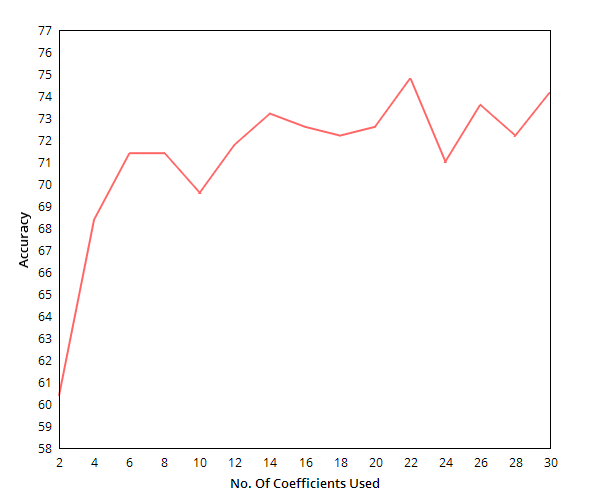
\includegraphics[width=170mm]{resources/mehang/6.4/MFCC_Num}
        \caption{Effect of number of MFCCs on result}
\end{figure}
The results indicate that once we use more than 10 MFCC Coefficients, the accuracy plateaus and doesn’t increase at all. So, using around 15 coefficients is found to be good enough for the problem domain.  

\newpage
\subsection{Analysis of Classifiers}
\subsubsection{SVM}
\paragraph{Selection of Kernels.}
\begin{figure}[h!]
        \centering
        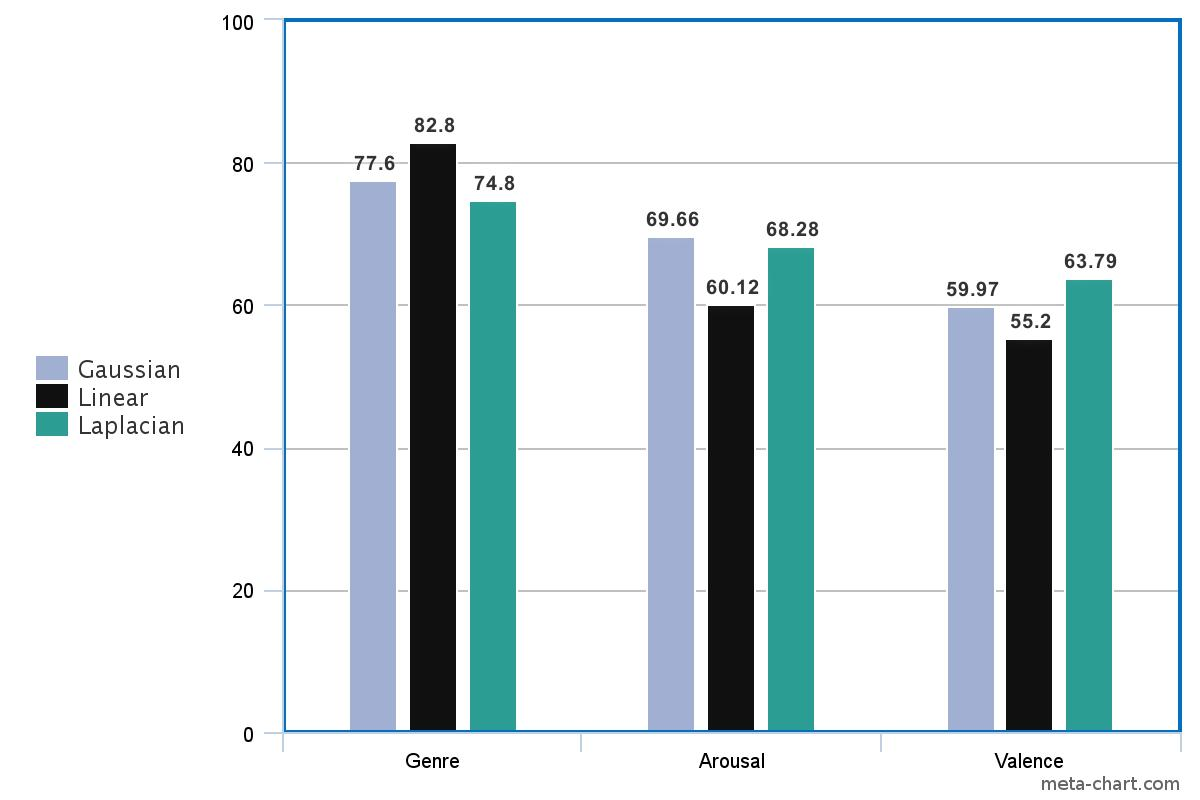
\includegraphics[width=170mm]{resources/mehang/6.5/SVM_Kernel}
        \caption{SVM Kernel}
\end{figure}

Linear Kernel performed best for the Genre Classification Problem and so we selected it for Genre Classification.\\
\\
As for the Mood Classification problem, both Gaussian and Laplacian out-performed the Linear Kernel in both arousal and valence classification. So, we selected Laplacian Kernel (based on its slightly superior performance) as our Kernel for Mood Classification.

\paragraph{Effect of Learning Iterations.}
We tested three iteration values to train SVM: one, 10 and 100.\\ 
\\
For Genre Classification, all three of them resulted in a similar performance of around 77 per cent accuracy.\\ 
\\
For Arousal, the performance increased when going from one (61 per cent) to 10 (69 per cent) iterations but increasing it further to 100 iterations didn’t increase the performance. We still received an accuracy of around 69 per cent.

\subsubsection{ANN}
\paragraph{Activation and Error Functions.}
We tried out two sets of Activation and Error Functions for the Neural Network with a 1000 iteration training.\\
\\
The results are given below:\\

\begin{table}[h!]
        \caption{Genre}
        \begin{center}
                \begin{tabular}{|l|l|l|l|}
                        \hline

                        Functions
                        &
                        Accuracy(percent)
                        &
                        Precision
                        &
                        Recall
                        \\\hline

ross Entropy Error with Softmax Activation
&
85.80
&
0.92
&
0.92
\\\hline

Least Mean Squares Error with Logistic Sigmoid Activation 
&
83.60
&
0.87
&
0.89
\\\hline
                 \end{tabular}
        \end{center}
\end{table}
So, the first combination slightly outperforms the second in all three metrics. 
\begin{table}[h!]
        \caption{Arousal}
        \begin{center}
                \begin{tabular}{|l|l|l|l|}
                        \hline

                        Functions
                        &
                        Accuracy(per cent)
                        &
                        Precision
                        &
                        Recall
                        \\\hline

                        Cross Entropy Error with Softmax Activation
                        &
                        69.31
                        &
                        0.72
                        &
                        0.64
                        \\\hline
                        
                        Least Mean Squares Error with Logistic Sigmoid Activation 
                        &
                        70.34
                        &
                        0.72
                        &
                        0.65
                        \\\hline

                 \end{tabular}
        \end{center}
\end{table}
\begin{table}[h!]
        \caption{Valence}
        \begin{center}
                \begin{tabular}{|l|l|l|l|}
                        \hline

                        Functions
                        &
                        Accuracy(per cent)
                        &
                        Precision
                        &
                        Recall
                        \\\hline

                        Cross Entropy Error with Softmax Activation
                        &
                        63.27
                        &
                        0.67
                        &
                        0.60
                        \\\hline
                        
                        Least Mean Squares Error with Logistic Sigmoid Activation 
                        &
                        64.31
                        &
                        0.68
                        &
                        0.60
                        \\\hline

                 \end{tabular}
        \end{center}
\end{table}

Here, the two combinations are almost inseparable in terms of performance. 

\paragraph{Number of Nodes in Hidden Layer.}

\begin{figure}[h!]
        \centering
        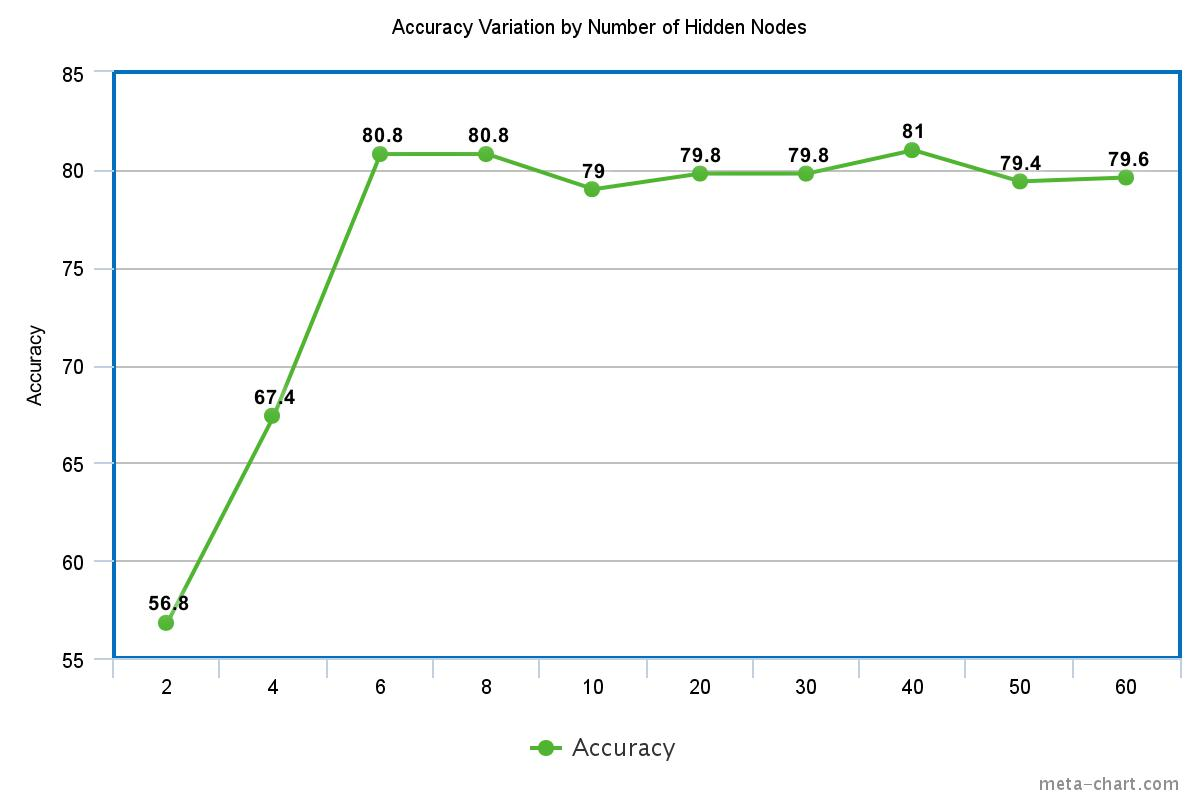
\includegraphics[width=170mm]{resources/mehang/6.5/ANN_HiddenNodes}
        \caption{Effect of number of hidden nodes}
\end{figure}

We used only one hidden layer as it should be enough for our problem domain. 
As seen in the figure, for any number of hidden numbers after six or so, we get almost the same accuracy. As a rule of thumb, it is usually recommended that the number of nodes be around the mean of the number of inputs and outputs, so we chose 30 as our final number of hidden nodes.\\
\\
The number of nodes had minimal effect in regard to mood classification. 

\paragraph{Number of Iterations.}
\begin{figure}[h!]
        \centering
        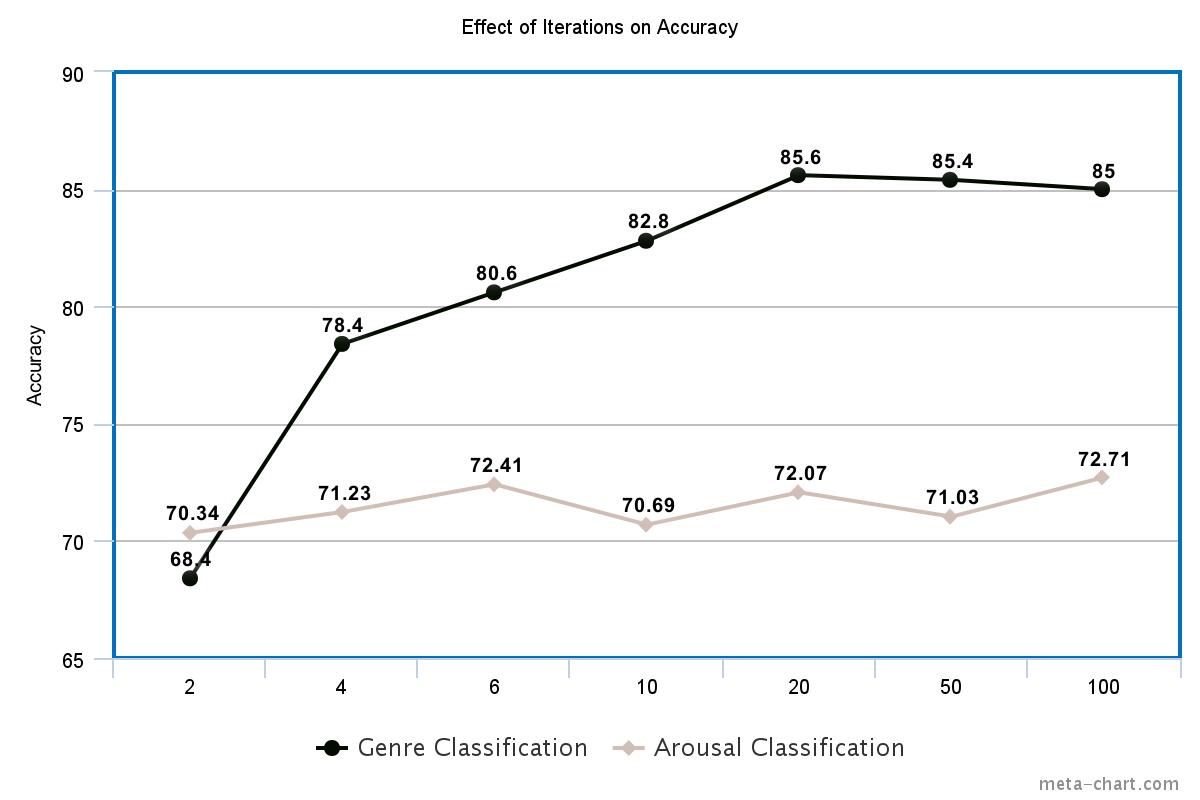
\includegraphics[width=170mm]{resources/mehang/6.5/ANN_Iterations}
        \caption{Effect of number of iterations}
\end{figure}
As seen in the figure, for genre classification, the number of iterations has an effect on the accuracy up to a certain point (around 20 iterations).\\
\\
As for Arousal, the increase in iterations had no effect on the accuracy. 

\newpage
\paragraph{Learning Rate.}
\begin{figure}[h!]
        \centering
        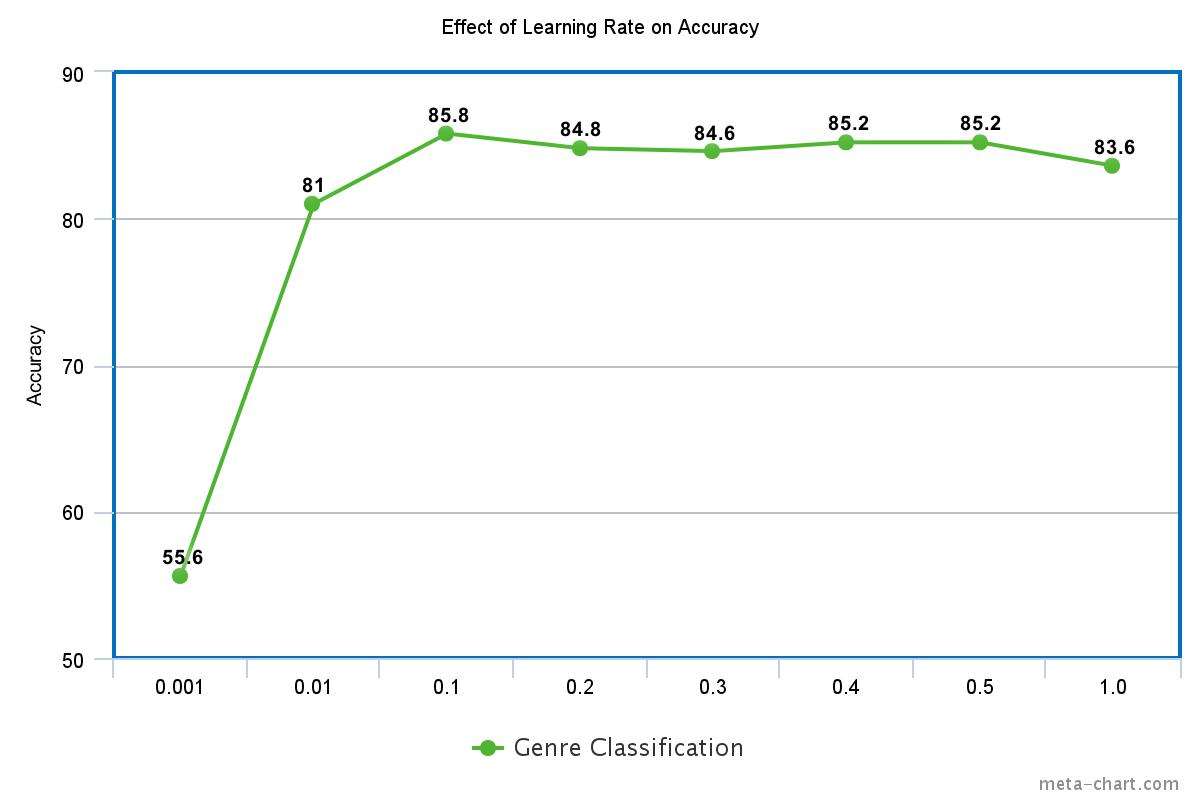
\includegraphics[width=170mm]{resources/mehang/6.5/ANN_Learning}
        \caption{Effect of learning rate}
\end{figure}

A learning rate of 0.1 was enough to get a decent amount of accuracy. A lower rate than that affected the accuracy while a higher rate didn’t have any influence at all.

\newpage
\subsection{Final Results}
\subsubsection{Genre Classification}
\begin{figure}[h!]
        \centering
        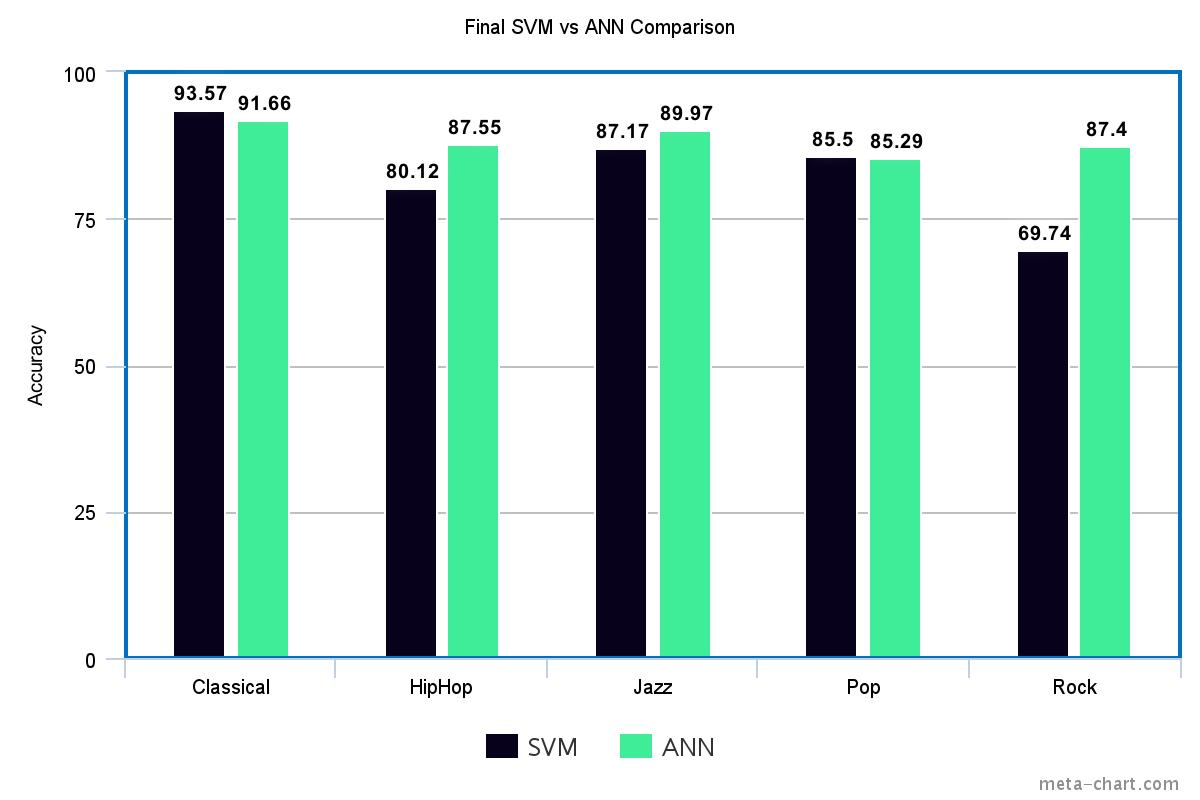
\includegraphics[width=130mm]{resources/mehang/6.6/FinalSVMANNGenre}
        \caption{Final SVM and ANN comparision based on genre}
\end{figure}

\begin{table}[h!]
        \caption{Genre classification performance measure}
        \begin{center}
                \begin{tabular}{|l|l|l|l|l|}
                        \hline

                        Classifier
                        &
                        Precision 
                        &
                        Recall 
                        &
                        F-Measure
                        &
                        Accuracy
                        \\\hline

                        SVM
                        &
                        0.87
                        &
                        0.94
                        &
                        0.89
                        &
                        83.00
                        \\\hline


                        ANN
                        &
                        0.94
                        &
                        0.92
                        &
                        0.92
                        &
                        88.80
                        \\\hline
                \end{tabular}
        \end{center}
\end{table}

For our final model we used ANN with these feature: MFCC, Spectral Centroid, Zero Crossing, Compactness and RMS.

\begin{table}[h!]
        \caption{Genre classification confusion matrix}
        \begin{center}
                \begin{tabular}{|l|l|l|l|l|l|}
                        \hline
                        &
                        Classical
                        &
                        Hiphop
                        &
                        Jazz
                        &
                        Pop
                        &
                        Rock
                        \\\hline

                        Classical
                        &
                        93
                        &
                        1
                        &
                        4
                        &
                        0
                        &
                        2
                        \\\hline

                        Hiphop
                        &
                        0
                        &
                        88
                        &
                        0
                        &
                        3
                        &
                        9
                        \\\hline


                        Jazz
                        &
                        5
                        &
                        0
                        &
                        90
                        &
                        1
                        &
                        4
                        \\\hline


                        Pop
                        &
                        2
                        &
                        7
                        &
                        0
                        &
                        86
                        &
                        5
                        \\\hline

                        Rock
                        &
                        0
                        &
                        4
                        &
                        4
                        &
                        5
                        &
                        87
                        \\\hline
                \end{tabular}
        \end{center}
\end{table}

\subsubsection{Mood Classification}
\begin{figure}[h!]
        \centering
        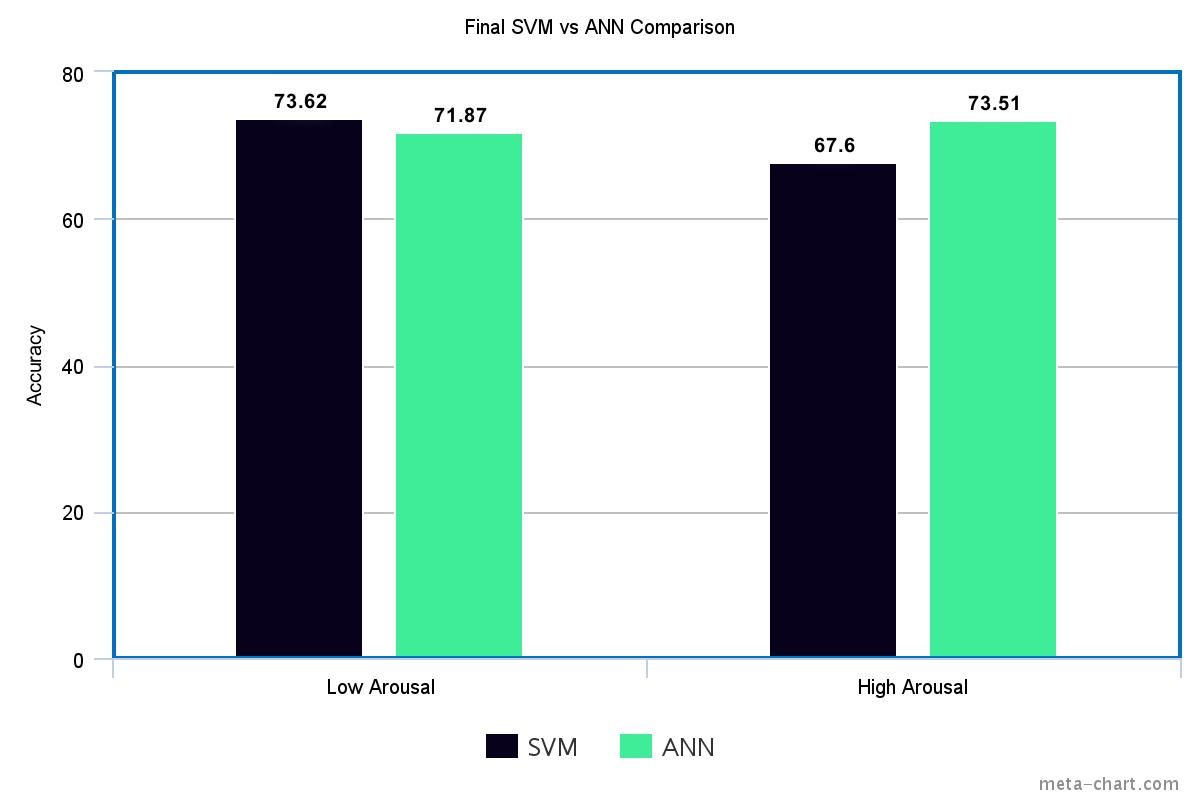
\includegraphics[width=130mm]{resources/mehang/6.6/FinalSVMANNArousal}
        \caption{Final SVM and ANN comparision based on arousal}
\end{figure}

\begin{table}[h!]
        \caption{Arousal classification performance measure}
        \begin{center}
                \begin{tabular}{|l|l|l|l|l|}
                        \hline

                        Classifier
                        &
                        Precision 
                        &
                        Recall 
                        &
                        F-Measure
                        &
                        Accuracy
                        \\\hline

                        SVM
                        &
                        0.70
                        &
                        0.74
                        &
                        0.72
                        &
                        70.69
                        \\\hline

                        ANN
                        &
                        0.75
                        &
                        0.72
                        &
                        0.72
                        &
                        73.10
                        \\\hline

                \end{tabular}
        \end{center}
\end{table}

For our final model we used ANN with these feature: Spectral centroid, MFCC, Zero Crossing, Compactness, Rhythm, Spectral Flux, RMS and Spectral Variability.

\begin{table}[h!]
        \caption{Arousal classification confusion matrix}
        \begin{center}
                \begin{tabular}{|l|l|l|}
                        \hline
                        &
                        Low Arousal
                        &
                        High Arousal
                        \\\hline

                        Low Arousal
                        &
                        105
                        &
                        40
                        \\\hline

                        High Arousal
                        &
                        38
                        &
                        107
                        \\\hline
                \end{tabular}
        \end{center}
\end{table}

\begin{figure}[h!]
        \centering
        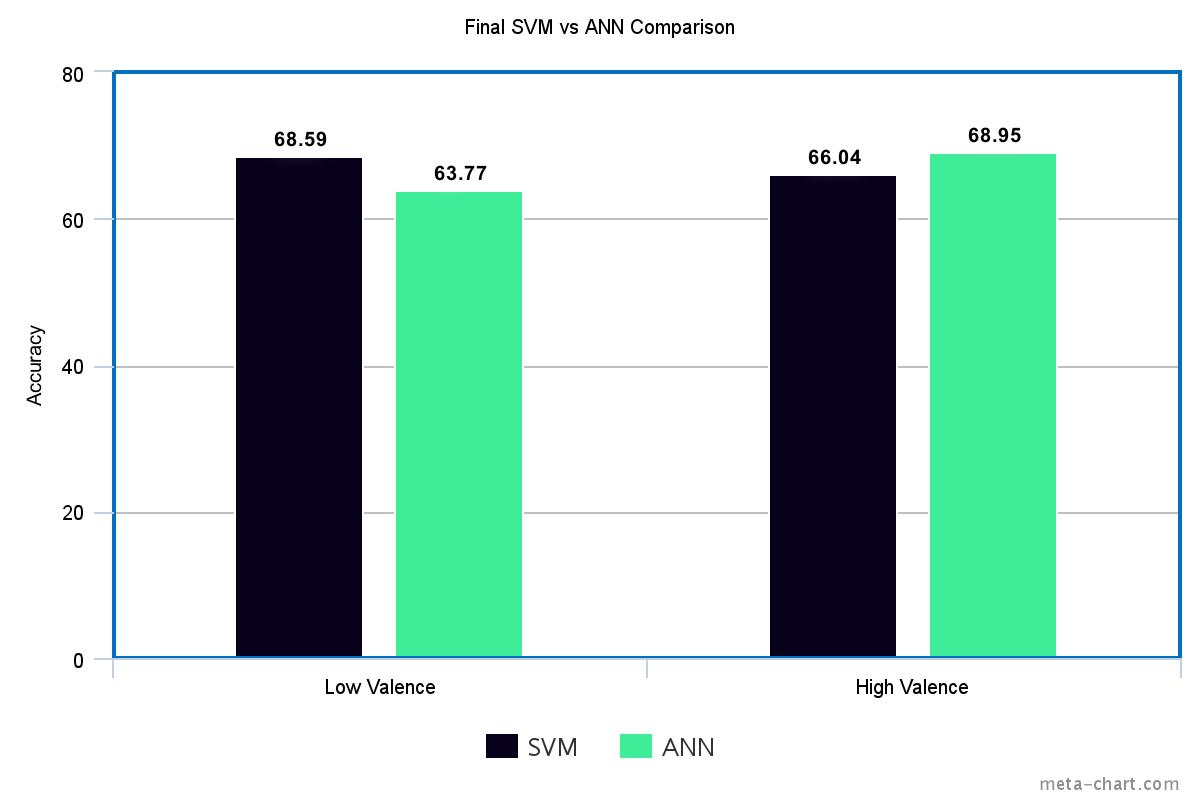
\includegraphics[width=130mm]{resources/mehang/6.6/FinalSVMANNValence}
        \caption{Final SVM and ANN comparision based on valence}

\end{figure}

\begin{table}[h!]
        \caption{Valence performance measure}
        \begin{center}
                \begin{tabular}{|l|l|l|l|l|}
                        \hline

                        Classifier
                        &
                        Precision 
                        &
                        Recall 
                        &
                        F-Measure
                        &
                        Accuracy
                        \\\hline

                        SVM
                        &
                        0.68
                        &
                        0.69
                        &
                        0.68
                        &
                        67.59
                        \\\hline

                        ANN
                        &
                        0.68
                        &
                        0.64
                        &
                        0.65
                        &
                        67.24
                        \\\hline

                \end{tabular}
        \end{center}
\end{table}

For our final model we used ANN with these feature: Spectral centroid, MFCC, Zero Crossing, Compactness, Rhythm, Spectral Flux, RMS and Spectral Variability.

\begin{table}[h!]
        \caption{Valence confusion matrix}
        \begin{center}
                \begin{tabular}{|l|l|l|}
                        \hline

                        &
                        Low Valence
                        &
                        High Valence
                        \\\hline

                        Low Valence
                        &
                        95
                        &
                        52
                        \\\hline

                        High Valence
                        &
                        43
                        &
                        100
                        \\\hline

                \end{tabular}
        \end{center}
\end{table}

\subsection{Problems and Solutions}
\subsubsection{Solved Problems}
\begin{enumerate}[(i)]
        \item \textbf{Mp3 Decoding:}The Mp3 file format uses various lossy compression techniques that allows it to store audio data in a compact and efficient manner. That however means that its headers and file formats are pretty complicated and decoding them would require a substantial amount of work. So, we had problems reading and decoding the Mp3 file format.\\ 
                \\
                We solved it by using the Mp3SPI library which read and gave us the samples of the mp3 files.
        \item \textbf{Feature Integration:}We had trouble deciding ways in which we could integrate the different song features into a single feature-set that could represent the song. This was complicated by the fact that the features all varied in length, range as well as magnitudes. 
                In the end, we concatenated the features into a single feature vector. However, by storing their means and standard deviation and normalizing them before usage, we minimized the effects of one feature over the others. 
        \item \textbf{Feature and Model Persistence:}We needed a way to store the extracted features and also the trained models. Doing so in a simple file or creating our own writer/parser for various appropriate formats would be error-prone and take up a lot of our time. 
                So, we used GSON and XStream to store and also read them as JSON and XML files respectively. 
        \item \textbf{Pitch Extraction:}Pitch is the perceived fundamental frequency and hence it is subjective. So, there is no definite mathematical formulae or methods to represent or calculate it. 
                So, we used the TarsosDSP library to extract pitch. 
\end{enumerate}

\subsubsection{Unsolved Problems}
\begin{enumerate}[(i)]
        \item \textbf{Distance Measure for Songs:} One way to achieve song clustering or even classification is to develop distance measures to figure out the ''distance'' or difference between any two given songs. So, we tried to do the same. However, our initial attempts at using a simple Euclidean Distance measure didn’t prove successful and later attempts using Gaussian Mixture Models proved to be too computationally intensive to be useful. 
        \item \textbf{Heap Error on Long Songs:}Due to lack of memory optimization we run into a Heap error when processing songs longer than about six minutes. This might be solved by better profiling of the memory used or by using shorter sections of songs for classification.
\end{enumerate}




\newpage

\section{CONCLUSION}
\subsection{Conclusion}
Automatic Music classification is an interesting problem that has gained prominence with the rise of the Internet and the subsequent growth in the amount of music available to the general populace.\\
\\
Any type of classification of music is difficult simply because the classifications themselves don’t have a clear definition. Still, we can work with fuzzy boundaries between these classes to get good enough results with Music Classification Systems.\\
\\
These systems broadly consist of two steps: Feature Extraction and Classification. However, they can be created by combining a variety of techniques and components.\\
\\
So, in this project, many such components and approaches were studied such as: types and combinations of features for proper representation of songs, feature integration approaches, classifier types, and their parameters, etc.\\
\\
All these studies were done in order to tackle two related but distinct problems: 
\begin{itemize}
        \item In Automatic Music Genre Classification (AMGC), very good performances were achieved with both of the classifiers employed: the final SVM model got 83 per cent accuracy and the ANN model getting 88 per cent accuracy for five genres. These results are comparable with the state-of-the-art results, especially involving the same dataset. 
        \item In Music Mood Classification however, the good results couldn’t be replicated. 
                The result along both axes of the music mood model used (arousal and valence) were underwhelming. Around 73 per cent accuracy was achieved using ANN for the binary low/high arousal classification. SVM did even worse with around 70 per cent accuracy. For low/high valence classification, both of the classifiers settled on 67 per cent accuracy.  
\end{itemize}

\subsection{Future Enhancements}
There are many ways in which the project could be expanded. 
\begin{itemize}
        \item Adding many more genres would be a natural enhancement as the five genres used here don’t even come close to encompassing all the variety of musical genres. 
        \item The mood model could also be made a continuum in the two-dimensional space instead of hard binary classifiers. 
        \item More features could be added to the feature set and studies conducted as to which combinations of features work best in which problem domain. 
        \item Smart Playlist Generation System could also be built using these types of Automatic Music Classification Systems. 
        \item The training set used to build the classifier could be increased in both size and variety to make the models generated more robust. This could also be a topic of study.
\end{itemize}







\newpage
\addcontentsline{toc}{section}{\numberline{}REFERENCES}
%\newgeometry{left=3.5cm,top=0cm,right=2cm,bottom=2cm}
\begin{thebibliography}{9}

        \bibitem{smith2013}
                Smith, Steven W.
                \emph{The scientists and engineers guide to digital signal processing.}
                California Technical Publishing, 2013. Print.

        \bibitem{muller2011}
                Muller, Mathias, et al. 
                \emph{Signal processing for music analysis.}, 
                Selected Topics in Signal Processing, IEEE Journal of 5.6 (2011): 1088-1110.

        \bibitem{dooling2014}
                Dooling, Robert J and Stewart H Hulse. 
                \emph{The Comparative Psychology Of Audition.} 
                Hillsdale, N.J.: L. Erlbaum Associates, 1989. Print.

        \bibitem{prasad2007}
                Prasad, Bhanu, and SR Mahadeva Prasanna, eds. 
                \emph{Speech, audio, image and biomedical signal processing using neural networks.} 
                Vol. 83. Springer, 2007.

        \bibitem{Neumayer2004}
                Neumayer, Robert. 
                \emph{Musical genre classification.} 
                (2004).

        \bibitem{Kour2015}
                Kour, Gursimran, and Neha Mehan. 
                \emph{Music Genre Classification using MFCC, SVM and BPNN.} 
                International Journal of Computer Applications 112.6 (2015).

        \bibitem{Koerich2013}
                Koerich, Alessandro L. 
                \emph{Improving the Reliability of Music Genre Classification using Rejection and Verification.} 
                ISMIR. 2013.

        \bibitem{Haggblade2011}
                Haggblade, Michael, Yang Hong and Kenny Kao. Music genere classification.
                \emph{Department of Computer Science},
                Stanford University,
                2011.

        \bibitem{Nasridinov2014}
                Nasridinov, Aziz, and Young-Ho Park. 
                \emph{A Study on Music Genre Recognition and Classification Techniques.} 
                International Journal of Multimedia and Ubiquitous Engineering 9.4 (2014): 31-42.

        \bibitem{Anglade2010}
                Anglade, Amélie, et al. 
                \emph{Improving music genre classification using automatically induced harmony rules.} 
                Journal of New Music Research 39.4 (2010): 349-361.

        \bibitem{LiTao2003}
                Li, Tao, and George Tzanetakis. 
                \emph{Factors in automatic musical genre classification of audio signals.} 
                Applications of Signal Processing to Audio and Acoustics, 2003 IEEE Workshop on.. IEEE, 2003.

        \bibitem{Tzanetakis1992}
                Tzanetakis, George, and Perry Cook, Musical genre classification 
                \emph{Journal of Personality},
                60(2):225–251,
                1992.

        \bibitem{Tzanetakis2002}
                Tzanetakis, George, and Perry Cook, Musical genre classification based on audio signals
                \emph{IEEE Transactions on Speech and Audio Processing},
                10.5 (2002)

        \bibitem{Apon2006}
                Apon, Amy, et al. 
                \emph{Inital Starting Point Analysis for K-Means Clustering: A Case Study.} 
                (2006).

        \bibitem{Jain2010}
                Jain, Anil K. 
                \emph{Data clustering: 50 years beyond K-means.} 
                Pattern recognition letters 31.8 (2010): 651-666.

        \bibitem{Hamerly2002}
                Hamerly, Greg, and Charles Elkan. 
                \emph{Alternatives to the k-means algorithm that find better clusterings.} 
                In Proceedings of the eleventh international conference on Information and knowledge management, pp. 600-607.
                ACM, 2002.

\end{thebibliography}


\clearpage
\appendix
\section*{APPENDIX A}
\addcontentsline{toc}{section}{\numberline{} APPENDIX A}
\setcounter{section}{8}
\subsection{Signal Processsing}
In signal processing, a window function (also known as an apodization function or tapering
function) is a mathematical function that is zero-valued outside of some chosen interval. For
instance, a function that is constant inside the interval and zero elsewhere is called
a rectangular window, which describes the shape of its graphical representation. When
another function or waveform/data-sequence is multiplied by a window function, the product
is also zero-valued outside the interval: all that is left is the part where they overlap, the
"view through the window".\\
\\
Applications of window functions include spectral analysis, filter design, and beam forming.
In typical applications, the window functions used are non-negative smooth "bell-shaped"
curves, though rectangle, triangle, and other functions can be used.
A more general definition of window functions does not require them to be identically zero
outside an interval, as long as the product of the window multiplied by its argument is square
integral, and, more specifically, that the function goes sufficiently rapidly toward zero.
One of the major applications of window functions includes the design of finite impulse
response filters and the spectral analysis.\\
\\
\subsection{Spectral Analysis}
The Fourier transform of the function cos ωt is zero, except at frequency ±ω. However, many
other functions and waveforms do not have convenient closed form transforms. Alternatively,
one might be interested in their spectral content only during a certain time period.
In either case, the Fourier transform (or something similar) can be applied on one or more
finite intervals of the waveform. In general, the transform is applied to the product of the
waveform and a window function. Any window (including rectangular) affects the spectral
estimate computed by this method.\\

\subsection{Windowing}
Windowing of a simple waveform like cos ωt causes its Fourier transform to develop non-
zero values (commonly called spectral leakage) at frequencies other than ω. The leakage
tends to be worst (highest) near ω and least at frequencies farthest from ω.
If the waveform under analysis comprises two sinusoids of different frequencies, leakage can
interfere with the ability to distinguish them spectrally. If their frequencies are dissimilar and
one component is weaker, then leakage from the larger component can obscure the weaker
one‟s presence. But if the frequencies are similar, leakage can render them irresolvable even
when the sinusoids are of equal strength.\\
\\
The rectangular window has excellent resolution characteristics for sinusoids of comparable
strength, but it is a poor choice for sinusoids of disparate amplitudes. This characteristic is
sometimes described as low-dynamic-range.\\
\\
At the other extreme of dynamic range are the windows with the poorest resolution. These
high-dynamic-range low-resolution windows are also poorest in terms of sensitivity; this is, if
the input waveform contains random noise close to the frequency of a sinusoid, the response
to noise, compared to the sinusoid, will be higher than with a higher-resolution window. In
other words, the ability to find weak sinusoids amidst the noise is diminished by a high-
dynamic-range window. High-dynamic-range windows are probably most often justified in
wideband applications, where the spectrum being analyzed is expected to contain many
different components of various amplitudes.\\
\\
In between the extremes are moderate windows, such as Hamming and Hann. They are
commonly used in narrowband applications, such as the spectrum of a telephone channel. In
summary, spectral analysis involves a tradeoff between resolving comparable strength
components with similar frequencies and resolving disparate strength components with
dissimilar frequencies. That tradeoff occurs when the window function is chosen.

\subsection{Filter Bank}
In signal processing, a filter bank is an array of band-pass filters that separates the input
signal into multiple components, each one carrying a single frequency sub-band of the
original signal. One application of a filter bank is a graphic equalizer, which can attenuate the
components differently and recombine them into a modified version of the original signal.
The process of decomposition performed by the filter bank is called analysis (meaning
analysis of the signal in terms of its components in each sub-band); the output of analysis is
referred to as a sub band signal with as many sub bands as there are filters in the filter bank.
The reconstruction process is called synthesis, meaning reconstitution of a complete signal
resulting from the filtering process.\\
\\
In digital signal processing, the term filter bank is also commonly applied to a bank of
receivers. The difference is that receivers also down-convert the sub bands to a low center
frequency that can be re-sampled at a reduced rate. The same result can sometimes be
achieved by under sampling the band pass sub bands.\\
\\
Another application of filter banks is signal compression, when some frequencies are more
important than others. After decomposition, the important frequencies can be coded with a
fine resolution. Small differences at these frequencies are significant and a coding scheme
that preserves these differences must be used. On the other hand, less important frequencies
do not have to be exact. A coarser coding scheme can be used, even though some of the finer
(but less important) details will be lost in the coding.\\
\\
The vocoder uses a filter bank to determine the amplitude information of the sub bands of a
modulator signal (such as a voice) and uses them to control the amplitude of the sub bands of
a carrier signal (such as the output of a guitar or synthesizer), thus imposing the dynamic
characteristics of the modulator on the carrier.\\

\newpage
\subsection{GUI}
\begin{figure}[h!]
        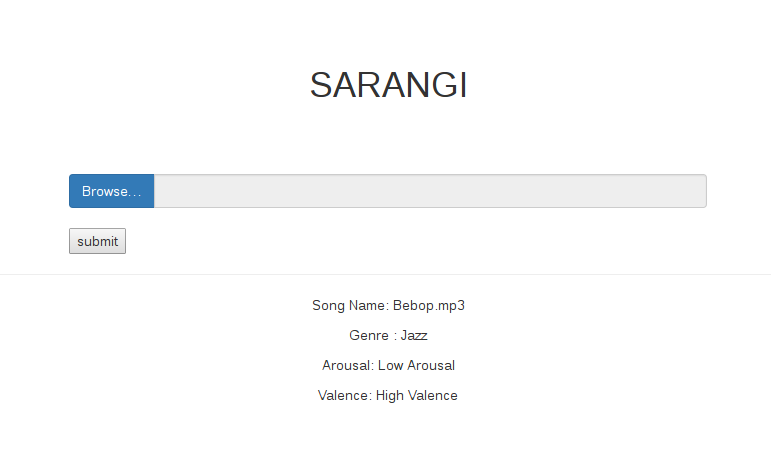
\includegraphics[width=150mm]{resources/gui}
        \caption{Graphical User Interface}
\end{figure}


\end{document}
